\documentclass[preprint,12pt]{article}

\usepackage{algorithmic}
\usepackage{algorithm}
\usepackage{enumerate}
\usepackage{enumitem}
\usepackage{graphics}
\usepackage{graphicx}
\usepackage{geometry}
\usepackage{amsmath}
\usepackage{wrapfig}
\usepackage{subfig}
\usepackage{framed}
\usepackage{color}
\usepackage{soul}
\usepackage{bm}

\usepackage{multirow}
\usepackage[T1]{fontenc}
\usepackage[latin9]{inputenc}
%\usepackage{units}
\usepackage{esint}
\geometry{legalpaper,  margin=1in}

\newcommand{\CM}[2][green]{ {\sethlcolor{#1} \hl{#2}} }
\newcommand{\KB}[2][cyan]{ {\sethlcolor{#1} \hl{#2}} }

%\makeatother

%\usepackage{babel}fs

\begin{document}
\title{An Empirical Bayesian Framework for Assessing Partisan Bias in Redistricting Plans}

\author{Kevin Baas and Colin McAuliffe}

\maketitle

\begin{abstract}
We present a framework for assessing partisan bias in redistricting plans using an empirical Bayesian approach, as well as a new metric for measuring partisan bias called the specific asymmetry.
Given at least one observation of the election results in a state, we estimate a probability model representing likely future election outcomes.
The expected value of the specific asymmetry is then computed by sampling from the model using the Monte Carlo method.
Redistricting plans which have an expected asymmetry of zero may be considered fair, since on average neither of the two major parties will be given an advantage.
Conversely, redistricting plans which have a nonzero expected asymmetry may be considered to be unfair, since partisan bias is a persistent feature of the plan.
Since this standard is symmetry-based it is consistent with previous supreme court opinions on partisan gerrymandering.
This analysis technique is applied to the United States congressional elections from 1972-2016 to examine the total and net effects of partisan bias in recent history.
We also examine the post 2010 census Wisconsin State Assembly, which is the subject of \emph{Whitford v. Gil}.

\end{abstract}

\section{Introduction}
In the United States, the process of drawing districts for a state's legislative bodies and federal congressional delegation is usually in the hands of that state's legislature.
Partisan state legislatures have used the redistricting process in pursuit of various goals such as incumbent protection, maximizing their share of seats, and even diluting the voting power of citizens on the basis of race.
Opportunities to manipulate the redistricting process for partisan advantage abound, particularly with the advent of sophisticated algorithms for redistricting as well as a high degree of partisan and geographic polarization in the current political climate.
However, the supreme court has yet to rule definitively on the issue of partisan gerrymandering, and recent rulings suggest that a manageable standard for measuring gerrymandering is a prerequisite for a such a ruling (LULAC v. Perry 2004).

The establishment of some standards to reel in partisan gerrymandering would have significant consequences for democracy in the United States.
Partisan gerrymandering not only distorts the composition of legislative bodies, it represents a dilution of the voter's ability to attempt to influence policy by electing representatives of their choosing.
The ability of state legislatures to use redistricting to influence the outcome of elections comes at the direct expense of voter's ability to use their ballot to influence the outcome of elections.
However, in order to properly asses the harm caused by partisan gerrymandering, courts require mathematical tools for analyzing partisan bias in a redistricting plan.

Development of a standard that fits with existing rulings, accurately measures partisan bias under generic conditions, and is simple enough to be effectively communicated to a court is not an easy task.
For example, a common sense standard might be to require that a party's share of seats is proportional to its share of votes, which is simple and applicable to swing states as well as more partisan states.
However, even when redistricting is fair, single winner voting systems tend not to produce such proportional outcomes \cite{Kendall_1950_10.2307/588113}, and the supreme court has stated that proportionality is not acceptable (Thornburg v. Gingles 1986).
A second example is the mean median difference test \cite{Wang__,Wang_2016_10.1089/elj.2016.0387,McDonald_2015_10.1089/elj.2015.0358}, which fits with existing rulings since it measures partisan bias without regard to proportionality and is simple enough to be calculated by a judge without an expert witness.
However, it is only effective in measuring bias for states which are close to even in terms of partisanship. \cite{Wang_2016_10.1089/elj.2016.0387}

Several standards have been proposed in literature, and for clarity we describe a standard as consisting of two parts.
The first part is a metric, which is some quantity that can be calculated from a given election result and is a measure of the unfairness or bias.
The second part is a model (or in the absence of a statistical model per se an analysis of the metric in historical elections), which allows one to asses whether or not the observed value of the metric can be regarded as the result of chance in an otherwise unbiased redistricting plan, or if bias is a persistent feature of the plan.
For example, the plaintiffs in Whitford v. Gil used a metric called the efficiency gap \cite{Stephanopoulos_2014_}, which measures the discrepancy in the so called wasted votes between the two major parties.
An examination of historical election data determined that it is reasonable to assume that observing an efficiency gap of greater than 7\% in favor of the redistricting party would typically be predictive of efficiency gaps favoring that party for the entire redistricting cycle.
Browning, Grofman and King proposed a metric based on the deficit in seats at 50\% votes in a seats votes curve \cite{Browning_1987_,Grofman_2008_}, which was used in a Bayesian model for evaluating redistricting plans in \cite{Gelman_1994_,Gelman_1994_a}.
Nagle has proposed several other metrics based on the seats votes curve \cite{Nagle_2015_10.1089/elj.2015.0311}, including the geometric area between the seats votes curve and its reflection, although no accompanying model was proposed.

A special group of standards are those where a particular metric is associated with an existing analytic statistical model.
Among these are the lopsided wins test, the mean median difference test, and the chi square test proposed by Wang \cite{Wang__,Wang_2016_10.1089/elj.2016.0387}.
These standards are attractive because they are based on statistics with properties that are well understood, that are used broadly for applications across many fields, and are relatively simple.
However, these tests have some drawbacks.
Namely, the models used for computing the significance level for those tests are valid asymptotically as the number of districts increases, meaning that the statistical power of these standards is diminished for states with just a few districts.
Additionally, a null distribution must be specified for each of the test statistics in question. 
This is a relatively minor point, since the null distributions used in the t-test and chi squared test are well established and the effect of the null distribution on the mean median difference test is small in many cases. \cite{Cabilio_1996_10.2307/3315744,Zheng_2010_}
\KB{I would argue its a major point.   And it's kind of subjective, anyways, whether its minor or major}
\CM{It's minor relative to the IID assumption. If IID is taken for granted then null distribution doesn't make much difference.}
Lastly and most importantly, these models assume that samples are independent and identically distributed (IID), which is an assumption that is crucial for the tests to be analytic (and hence simple) but not necessarily realistic for elections.
For instance, the IID assumption would imply that the probability of a deeply partisan Republican district being won by a Republican is the same as the probability of a deeply partisan Democratic district in the same state being won by a Republican.
Violation of the IID assumption can have a noticeable effect on statistical tests, for an example in securities law see \cite{Gel_2009_10.1093/lpr/mgp008}. 
Use of this assumption may make this group of standards too restrictive or too permissive depending on the specific circumstances.
Despite these objections, standards based on analytic models are potentially very powerful due to their relative simplicity and their ability to be solved without sophisticated analysis.
We are currently investigating the effect the IID assumption has on the robustness of such standards.

Another group of standards are those based on Monte Carlo simulation.
A major advantages of Monte Carlo based standards are flexibility, since they do not require the metrics to be analytically integrable, and thus can be used with a wide variety of metrics or even multiple metrics in combinations.
Additionally, once implemented by a computer algorithm, it is quick and easy to look at the data in many different ways.

An example is test III proposed by Wang \cite{Wang__,Wang_2016_10.1089/elj.2016.0387}, where the metric used was the proportion of seats won by a party, and the model was a Monte Carlo technique where 'fantasy' congressional delegations were sampled from national congressional voting results.
This method can be used to establish whether or not a party's vote share wins them seats excessively relative to a national baseline.
A second example of a Monte Carlo based standard is that of Chen et al \cite{Chen_2015_10.1089/elj.2015.0317,Chen_2016_10.1016/j.electstud.2016.06.014}, where electoral maps satisfying basic redistricting criteria are generated randomly and compared against the actual map.
The standard that we propose is also based on Monte Carlo simulation.
The metric, which we refer to as the specific asymmetry (see section \ref{sec:MB}), is a measure of partisan bias that determines discrepancy in seats won by the losing party under a reversal in statewide partisanship.  
The model, described in section \ref{sec:FB}, uses a Monte Carlo technique based simulations of an empirically estimated probability model for district and statewide partisanship.
The drawback of Monte Carlo based standards is complexity relative to analytic standards which do not require a computer to implement.
Since Monte Carlo is a numerical integration method, as opposed to analytic, it take a lot more computer processing power, and thus aren't as well suited for use in optimization algorithms, relative to analytic methods.
Nonetheless, Monte Carlo simulation techniques are highly conventional tools that are in widespread use across numerous disciplines \cite{Kroese_2014_10.1002/wics.1314}, and are useful for examining bias in redistricting.

The empirical Bayesian framework that we propose is not only appropriate for assessing bias that has existed in past redistricting plans, but it is useful for understanding how bias could be introduced into future redistricting plans, even as strategies for gerrymandering change in response to the introduction of a hypothetical standard.
In fact, the empirical Bayesian model that we propose is compatible with all of the metrics we have discussed thus far, and can be used as part of a standard itself, or can be used to test the robustness of standards that do not require Monte Carlo simulation. 
We therefore contend that regardless of whether or not the approach we present is an acceptable judicial standard itself, it remains a powerful tool for assessing partisan bias in redistricting plans that will prove useful for researchers and advocates of redistricting reform.
For example, the Monte Carlo technique can be used to evaluate the properties of metrics which do not have well known analytic statistical properties such as the efficiency gap and the specific asymmetry metric proposed in section \ref{sec:MB}, or to evaluate the effect of the IID assumption for metrics which do have known analytic properties such as the mean median difference and the t-test.
Additionally, the technique could be used to help develop an understanding of the conditions where different metrics may agree or disagree with one another.
For fast reference, table \ref{tab:Stand} summarizes each of the standards discussed here. 

\begin{table}[htb!]
\centering
\caption{Summary of the metrics and models employed by various gerrymandering standards \label{tab:Stand}}
\begin{tabular}{|l|l|l|}
\hline
Standard & Metric & Model\\
\hline
\hline
Grofman and King & Deficit in Seats at 50\% of the vote & None proposed\\
\hline
Nagle & Various metrics of seats & None proposed\\
      & votes curve asymmetry &  \\
\hline
Stephanopolous and McGhee & Efficiency gap & None proposed,\\
                          &                & historical analysis used\\
                          &                & in \emph{Whitford v. Gil}\\
\hline
Gelman et al & Deficit in Seats at 50\% of the vote, & Bayesian simulation\\
             & various others & \\
\hline
Mean Median Difference & Mean median difference & asymptotic distribution \\
 &                                              & (unit normal) \\
 &                                              & assuming IID samples \\
\hline
Chi square test & Party in state and national  & asymptotic distribution  \\
                & winning vote share variances  & (chi squared) \\
                &   & assuming IID samples \\
\hline
Lopsided wins test & Difference in party  & asymptotic distribution  \\
                   &  mean winning vote share & (student's t) \\
                   &   & assuming IID samples \\
\hline
Test III \cite{Wang_2016_10.1089/elj.2016.0387} & Party seat share & MC sampling of national \\
or 'excess seats test'         &                  & district voting results\\
\hline
Chen and Rodden & Party seat share & MC sampling of randomly \\
         &                         & generated districting plans\\
\hline
Present study & Specific Asymmetry & MC sampling of the \\
              &                    & empirical Bayesian model\\
\hline
\end{tabular}
\end{table}

\section{Measuring Bias with the Specific Asymmetry\label{sec:MB}}

Measuring partisan bias accurately presents several challenges from a mathematical and legal perspective.
Redistricting will always be an artificial process, and therefore we must establish what characteristics of a redistricting plan can be regarded as normative before attempting to measure deviations from the normative standard.
We propose the following definition: \emph{a fair redistricting plan is one that, on average, will not be biased in favor of either of the two major parties}.
With this definition in mind, we turn our attention to several challenges in devising a metric for bias.
First, single winner elections tend not to produce proportional outcomes \cite{Kendall_1950_10.2307/588113}, and we therefore can not use proportionality or the lack thereof as a measure of bias.
Bias should therefore be a measure of symmetry, which permits disproportionate outcomes but requires that any advantage that might arise from the disproportionate nature of the single winner election system be equally available to either party.
In other words, we say that the result is unbiased if and only if any advantage gained by a party, above what is proportional, is a consequence of the disproportionate nature of the single winner election system, and not an additional advantage piled on top of that.

A few measures of bias that follow this definition exist in the literature, such a Grofman and King, and the mean median difference \cite{Grofman_2008_,Wang__,Wang_2016_10.1089/elj.2016.0387}.
However, these measures of bias tend to apply only to states which are close to 50-50 partisanship.
For more partisan states, these measures become more difficult to interpret except as the bias which could have occurred had the partisanship in the state in question been closer to even.
Another approach is to consider the bias at levels of partisanship by using the geometric area between the seats votes curve and its reflection \cite{Nagle_2015_10.1089/elj.2015.0311}.
Useful information may be gleaned from these approaches, but Justice Kennedy expressed a dislike for measures based on a hypothetical state of affairs.
Additionally, measurement of bias at different levels of hypothetical partisanship may lead to significantly different results depending on the partisanship level considered.
For example, the seats votes curve for the Wisconsin state assembly shows substantial bias favoring Republicans at close to even partisanship, but the complete reverse at high levels of Democratic partisanship.
This means that bias measures which do not consider the actual partisanship in a state could result in false positives and false negatives.
In light of this, a measure of bias that is applicable to any level of partisanship and that directly considers the actual level of partisanship in a given state seems appropriate.

To address these challenges, we propose a measure of bias which we call the specific asymmetry, which is the deviation of the seats votes curve from the symmetry line measured at the statewide popular vote.
This amounts to counting the number of seats won by one party, then counting the how many seats the other party would win under a uniform partisan swing that reverses the statewide partisanship.
The specific asymmetry is then the difference between these two seat counts divided by two.
This definition of partisan asymmetry simply requires that the seat count to reverse along with a reversal in the popular vote in a state.
This has a certain intuitive appeal and is consistent with existing law since disproportionate results are allowed, as long as both parties are treated the same.
However, one may argue that a reversal of the popular vote is a unrealistic counterfactual scenario that is beyond the scope of any sensible analysis technique.
This is true in the sense that we could not predict what the distribution of votes would be if such a partisan reversal would actually occur, but it is important to note that when we compute the discrepancy in seat counts under a uniform reversal in statewide partisan ship, we are computing the magnitude of structural disadvantage faced by the voters of one party.
In other words, while the specific asymmetry may be phrased as a sort of hypothetical, it measures a \emph{real} electoral disadvantage endured by one party resulting from that party winning seats less efficiently than the opposite party due to voter packing and cracking.
Further, as the magnitude of the structural disadvantage to one party increases due to a more aggressive gerrymander, the specific asymmetry increases as well.
There are several other advantages to using this metric, which we summarize below.

\begin{itemize}

\item It doesn't assume proportionality in results - The seats-votes curve for single-winner elections naturally takes on a cumulative Beta-binomial distribution, as opposed to a diagonal line representing seats proportional to votes.  This metric doesn't assume a diagonal curve representing proportionality.  It tests a looser (less strict) criteria: asymmetry, which still retains the essential feature of measuring disenfranchisement based on political belief.  SCOTUS has ruled that seats proportional to votes can not be a legal standard (Thornburg v. Gingles 1986).   However they remain open to a legal standard based on the idea of partisan symmetry (LULAC v. Perry 2004).
 
\item It distinguishes between artificial partisan bias and the natural multiplying effect of single-winner elections -  Single-winner aka "Majoritarian" elections naturally over-favor the majority party, giving them a larger fraction of the seats than their fraction of the popular vote.  
While some measures might mistakenly identify this as gerrymandering, specific asymmetry explicitly takes this into account by calculating and then subtracting this natural multiplying effect.

\item It works for states with partisanship far from 50/50 - By sampling the asymmetry at the actual vote counts rather than e.g. 50/50, this metric maintains full relevance even for the most extremely partisan states.

\item It represents deviation from what is practically achievable - It is trivial for a computer algorithm to design districts that make the seats-votes curve perfectly symmetric, while satisfying all constitutional requirements.  
Thus, to convert this absolute score to one relative to what can be accomplished by a redesign that meets all traditional redistricting principles, one simply subtracts zero.  
This "new" relative score gives you the number of voters whose votes were effectively stolen by the map drawers with the current map, and whose right to representation can be returned by a remedy map that can be trivially designed by a computer employing a multi-objective heuristic optimization algorithm.

\item The only possible improvements to it are shift, scale, and shape - Since it is well ordered and monotonic with respect to actual partisan advantage, any "better" measure can only be better in the sense of having a more appropriate "center" point, a more appropriate scale, or a more appropriate "shape" (change of slope as you go up and down the scale).  The scale varies from -1 to 1, or alternatively from negative the number of seats available to the positive of that.  The "center",  zero, is a non-arbitrary and very reasonable choice, representing a perfectly symmetric situation.   The "shape" is the number (or percentage) of congressional seats affected.

\item It gives a result in an empirically meaningful unit: number of seats, which can be directly converted into number of ballots/voters affected by multiplying by the number of ballots cast and dividing by the number of districts.

\end{itemize}

Bias by any measure may occur by chance in an otherwise fair redistricting plan, it is even possible for an antimajoritarian outcome to result from chance.
It is also important not only to consider the harm a plan has caused to voters, but to also seek to assess the likelihood that a plan will cause harm to voters in future elections.
For example, the plaintiffs in \emph{Whitford v. Gil} argued that based on an examination of a large body of election data, an observed efficiency gap of greater than 7\% in a given election was strongly suggestive that bias in favor of the redistricting party would persist.
In other words, the observation of a large bias was not only indicative of harm to voters that had already occurred, but it was also a strong predictor of likely future harm to voters.
Analysis of historical data is not the only way to assess likely future harm due to bias, and we would like to use a method that takes advantage of as much specific information about the redistricting plan in question as possible.
Therefore we employ an empirical statistical model to determine whether a particular redistricting plan will be biased or unbiased \emph{on average}.
Full details of the particular model employed here are presented in the following section.


\section{Modeling the Likelihood of Bias in Future Elections\label{sec:FB}}

We can measure bias in a single election with the specific asymmetry, but we would also like to know the chances that a given redistricting plan will lead to bias in future elections.
This allows us to distinguish between chance occurrences of asymmetry on an otherwise fair map and maps for which asymmetry is a persistent feature.
A particular election result represents one possible outcome among many outcomes that could have occurred, or in other words each election represents a sample from a population representing all possible election outcomes.
We can use the observation of one or more elections along with prior knowledge of election data to make inferences about the population.
To this end we estimate parameters for a statistical model representing partisanship in each district as well as statewide partisanship given at least one election result in a state.
Each sample drawn from this model represents a plausible election result that could have occurred if we were able to rerun elections as many times as we wanted.
For each sample, we compute the specific asymmetry and the mean asymmetry of all samples giving the expected specific asymmetry, as well as other descriptive statistics representing the likelihood of different levels of asymmetry.
Thus, the proposed definition that \emph{a fair redistricting plan is one that, on average, will not be biased in favor of either of the two major parties} corresponds to a map with an expected asymmetry of zero.
The details of the empirical Bayesian model are outlined in what follows.

\subsection{Model Parameterization}
To chose a model appropriately, we must carefully consider the underlying process. 
The Beta distribution is a natural choice for many processes that involve percentages, and is appropriate for modeling election outcomes. 
This choice of probability model for modeling an election is not new. 
It has been used in numerous academic papers, and continues to be used in literature published quite recently \cite{Paolino_2001_,Kaplan_2003_10.1287/opre.51.1.32.12794,Murr_2015_10.1177/2053168015583346}.
Indeed, teaching materials about the Beta distribution often use elections as an example.  
Some academic papers have extended this model to take into account third parties by using the Dirichlet distribution \cite{Rigdon_2009_10.1177/1532673X08330670} (The Dirichlet distribution is the multivariate extension of the Beta distribution.) 

The choice of the Beta distribution follows directly from first principles. 
In fact, two different points of view of the underlying stochastic process of election results both lead us to the Beta distribution. 
In the first point of view, we can consider the underlying stochastic process is a Bernoulli process, which a number of trials that can each have one of two outcomes, i.e. a Republican vote or a Democratic vote.
We are interested in the number of votes for a given party out of all the votes, which is the number of successes in a sequence of trials.  
This leads us to the Binomial distribution. 
However, we do not know the rate of 'successes' (or the votes for an arbitrarily selected party), that is what we are trying to estimate.  
To estimate the rate parameter of a Binomial distribution, we use its conjugate prior distribution, which is the Beta distribution.

Depending on our point of view, the or   

In the second perspective voting is considered a pair of Poisson processes, which are series of events occurring at a certain rate i.e. voters for a party turning out to cast a vote. 
Here we are interested in the number of times a voter for a party turns out to vote in a given amount of time (Election day) - the number of events in a fixed interval. 
This leads us to the Poisson distribution.  
However, we do not know the rate of events - that is what we are trying to estimate.  
To estimate the rate parameter of a Poisson distribution, we use its conjugate prior distribution, which is the Gamma distribution. 
To represent partisanship as a fraction, we take the fraction of events between the two Poisson processes.  
Let $\Gamma\left(X\right)$ be the unknown rate of voter turnout for one party, and $\Gamma\left(Y\right)$ the unknown rate for the other.
The proportion of votes won by party X is $\frac{\Gamma\left(X\right)}{\Gamma\left(X\right)+\Gamma\left(Y\right)} $. 
This leads us to the Beta distribution.
Thus, deduction from first principles leads us to select the Beta distribution as our probability model for the outcome of an election, regardless of which perspective we initially take.
With the choice of model parameterization in hand, we now turn our attention to estimation of the parameters for the beta distributions representing district and state partisanship.

\subsection{Parameter Estimation}
The shape parameters for the beta distributions for district partisanship are estimated using the method of moments as follows
\begin{equation}
    \alpha = \bar{x} \left(\frac{\bar{x}\left(1-\bar{x}\right)}{\bar{v}}-1\right)
\end{equation}
\begin{equation}
    \beta = \left(1-\bar{x}\right) \left(\frac{\bar{x}\left(1-\bar{x}\right)}{\bar{v}}-1\right)
\end{equation}
where $\bar{x}$ is the district mean vote percentage and $\bar{v}$ is the variance of the district vote percentage.
A practical challenge to using these formulas is that at most five data points will be available for a given district in a redistricting cycle.
Often, fewer data points may be available if a redistricting cycle is not yet complete or if a district had uncontested elections.
To make use of the model when only one data point is available and to help reduce the effects of small sample sizes in the parameter estimation process, we use a shrinkage term when computing the district variance $\bar{v}$ for N observed elections as follows

\begin{equation}
    \bar{v} = \frac{1}{N}\left[\sum_{n=1}^{N}\left(x_{n}-\bar{x}\right)^{2}+\hat{v}\right]
\end{equation}
where $\hat{v}$ is the shrinkage variance which can be set based on historical data.
Note that if there is only one data point available the variance is simply the shrinkage variance, without which the variance would be undefined.

To obtain $\hat{v}$, we use the average sample variance of district partisanship in contested elections over all districts and cycles.
This is show in figure \ref{fig:varHist}, where we obtain an average variance of .529\% (corresponding to a standard deviation of 7.26\%) over all cycles.
The within cycle average could also be used as the shrinkage variance, to attempt to capture trends in political polarization.

\KB{I noticed you changed this from average standard deviation to average variance, and that it changes the result slightly. (0.00529 instead of 0.0037)  not sure which way is better...}\CM{Yes I used variance because that's what used in the method of moments formula}\KB{I think it makes sense.}
\begin{figure}[htb!]
    \begin{center}
        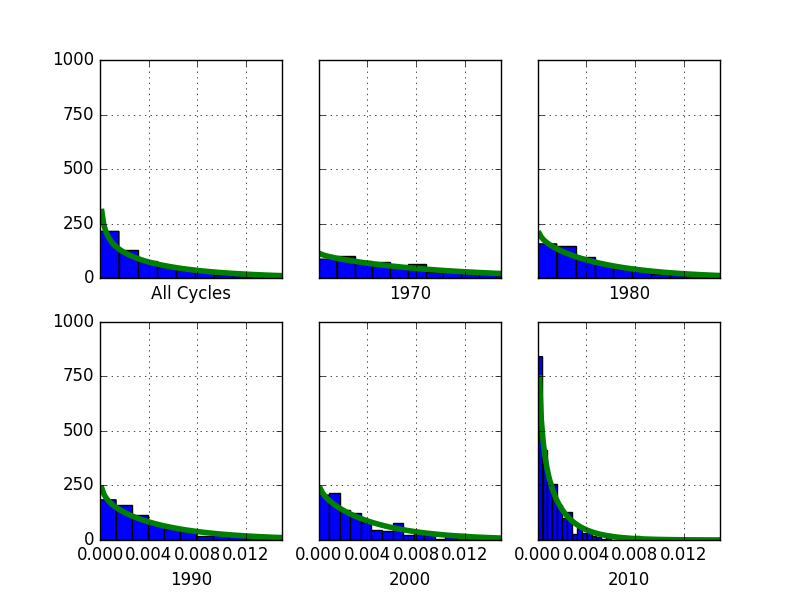
\includegraphics[scale=0.8]{../Figures/HistoricAsymmetry/VarHist.png}
        \caption{Distribution of sample variance of district partisanship over contested elections in each cycle. The green lines are the result of fitting the variances to a beta distribution}\label{fig:varHist}
    \end{center}
\end{figure}
\subsection{Model Integration}
To compute the expected specific asymmetry, we use Monte Carlo sampling.
One sample from the model involves taking one sample from each district and one sample for the popular vote.
Seat counts can then be tallied along with various measures of bias and competitiveness.
We then compute the average specific asymmetry over all samples along with other descriptive statistics.
This approach has several advantages

\begin{itemize}

\item Non-uniform swings are accounted for. Accounting for the average partisanship of each district as well as the variance in partisanship from election captures the changes in voter sentiment that are not uniform throughout the state.

\item It takes into account all possibilities, weighted by likelihood - Every possible seats-votes curve and every possible popular vote ratio is taken into consideration, weighted by the combined likelihood of the two.

\item It shows durability - By computing an entire likelihood function for specific partisan asymmetry, rather than a single point estimate, this approach enables quick and accurate assessment of how durable a gerrymander is. This gives us insight into how much more harm it will cause in the future, including what the likelihood is that it will not cause harm.

\end{itemize}

To illustrate the process we show a few samples from this model for the Wisconsin state assembly districts figure \ref{fig:SVAssembly2010} (a full analysis of this districting plan can be found in section \ref{sec:Wis}).
The dark line is the seats votes curve generated from sampling the partisanship in each district, while the dashed line in the reflection of this curve.
Discrepancies between these two lines represent asymmetries, which vary depending on the level of partisanship considered.
The vertical line is the statewide partisanship sampled from the state beta distribution, which determines the partisanship level that we measure the asymmetry at.

\begin{figure}[htb!]
    \begin{center}
        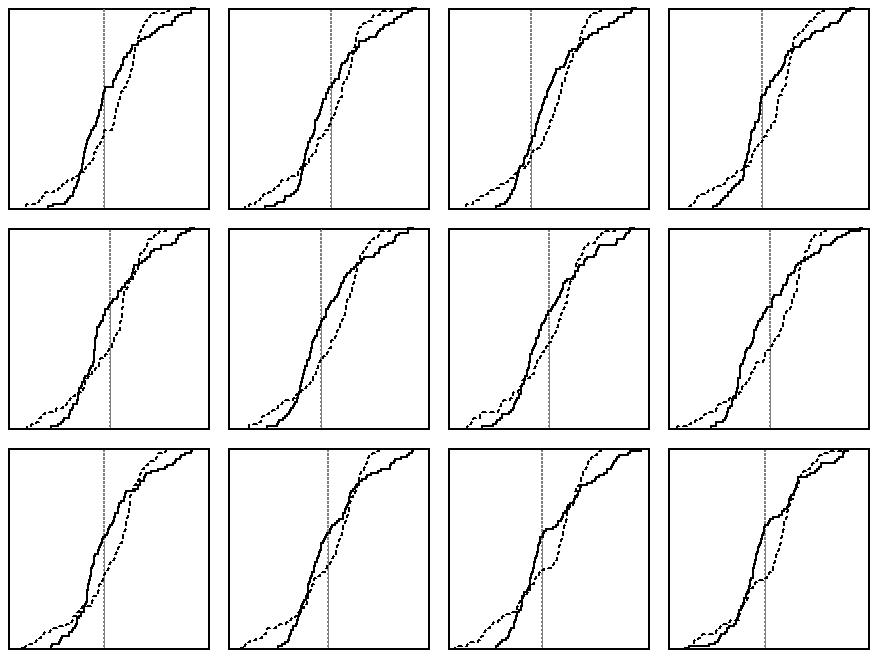
\includegraphics[scale=0.45]{../Figures/WI2010/sv_curves_assembly.png}
        \caption{Some election outcome seats-votes curves generated from the probability model for Wisconsin 2010 Assembly districts}\label{fig:SVAssembly2010}
    \end{center}
\end{figure}

\section{Partisan Bias in the U.S. Congress 1972-2016\label{sec:Hist}}
We present an examination of partisan bias in the United States congress for elections from 1972 to 2016.
The election data were collected by Brian Remlinger and Sam Wang, and sent to us in a personal communication.
First, to illustrate the effect of asymmetry on the composition of congress, we compute the specific asymmetry for each state and election, and compare the Democratic popular vote share to the actual Democratic seat share as well as the Democratic seat share that would have resulted if each election had zero asymmetry.
This illustrates a few of the features of the specific asymmetry as a metric, but we note that this is not exactly representative of how the composition of congress would have been different had the proposed standard been enforced in each of these redistricting cycles.
The reason for this is that the proposed standard would enforce an expected asymmetry of zero, meaning on average no asymmetry would occur but in some elections asymmetry could occur by chance.
This result is shown in figure \ref{fig:AsymRemoved}, where it is evident that despite the natural multiplying effect of majoritarian elections, removing specific partisan asymmetry produces congressional representation closer to proportional with the popular vote, regardless of which party the net partisan asymmetry favors.  
Thus while proportionality of seats and votes is not enforced, gerrymandering tends to exacerbate and amplify the natural tendency of single winner elections to lead to disproportionate representation in favor of the majority party, and therefore removal of asymmetry caused by redistricting tends to lead to results that are closer to proportional.
If one were to use a metric that assumes votes should be proportional to seats, such as the efficiency gap, the 1970s would still be counted as gerrymandered, despite all partisan asymmetry being removed.  
That is, efficiency gap would mistake the unavoidable multiplying effect of the sigmoidal seats-votes curve for gerrymandering.\CM{I'm not sure about this, the eg does assume proportionality but it does not assume that the constant of proportionality between seats and votes is 1} \KB{not assuming a proportion of 1 doesn't make it sigmoidal}\CM{That's true but I think the claim you make requires seats = votes and would not neccisarily hold up for the more general seats ~ votes}
Specific partisan asymmetry, however, never makes this error, while still leading to a substantial increase in the representativeness of congress as a whole.

\begin{figure}[htb!]
    \begin{center}
        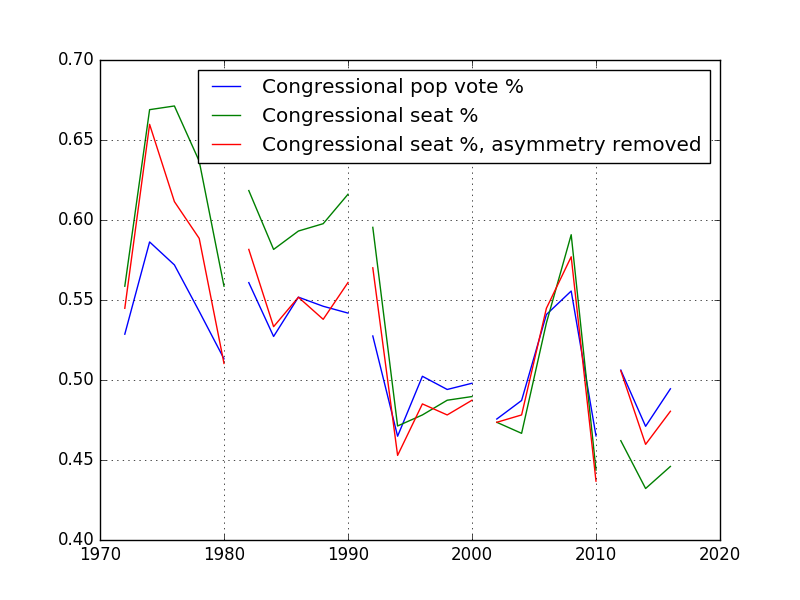
\includegraphics[scale=0.8]{../Figures/HistoricAsymmetry/sv.png}
        \caption{Democratic vote share and seat share with asymmetry removed 1972-2016}\label{fig:AsymRemoved}
    \end{center}
\end{figure}

Next we account for random variability in the results by computing expected specific asymmetry for each state and redistricting cycle using 10,000 Monte Carlo samples.
First, we consider the net asymmetry, which is indicative of how gerrymandering may have affected the partisan composition of congress.
In figure \ref{fig:NetAsym}, the net observed asymmetry is shown for each election.
The expected net asymmetry for each redistricting cycle is also shown with 50\% and 90\% confidence intervals.
A progression is observed where the net asymmetry strongly favored Democrats in the 70's and 80's, mildly favored Democrats in the 90's, was roughly zero net asymmetry in the 2000's, and strongly favored Republicans in the 2010 cycle.
Histograms for the simulations can be found in figure \ref{fig:NetAsymHist}, which shows the expectation and variance of the net specific asymmetry.
In the 80's for example, Democrats could expect about 20 seats on average due to redistricting bias, with a negligibly small probability that the net national asymmetry would favor Republicans.
This situation has reversed entirely by the 2010 cycle, where Republicans can expect 18 seats on average due to redistricting bias.
Interestingly the 2000's show zero net bias on average, but this does not mean that the country was free of gerrymandering.
As we will show later in this section, there was significant gerrymandering by Republicans and Democrats in their respective territories, but the net effect of these gerrymanders tended to roughly cancel.
\begin{figure}[htb!]
    \begin{center}
        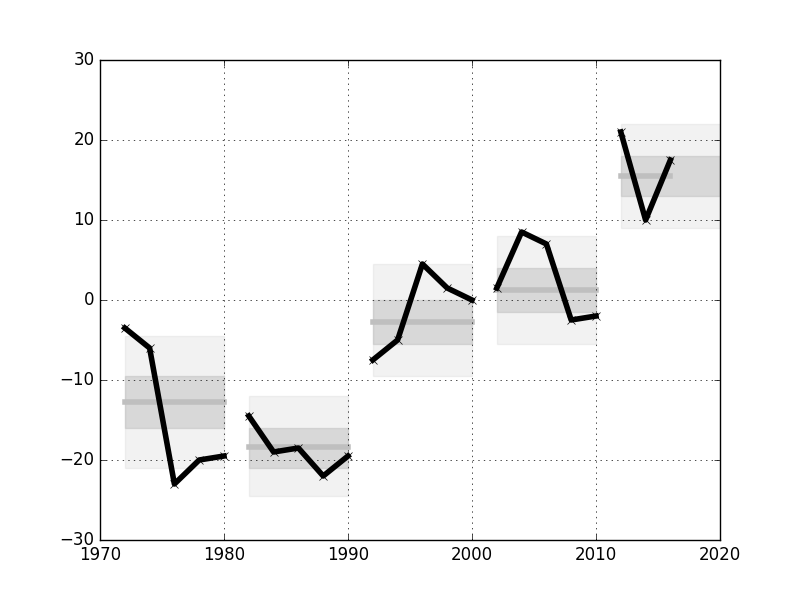
\includegraphics[scale=0.8]{../Figures/ExpectedAsymmetry/netAsym.png}
        \caption{Net national asymmetry based on 10,000 simulations}\label{fig:NetAsym}
    \end{center}
\end{figure}
\begin{figure}[htb!]
    \begin{center}
        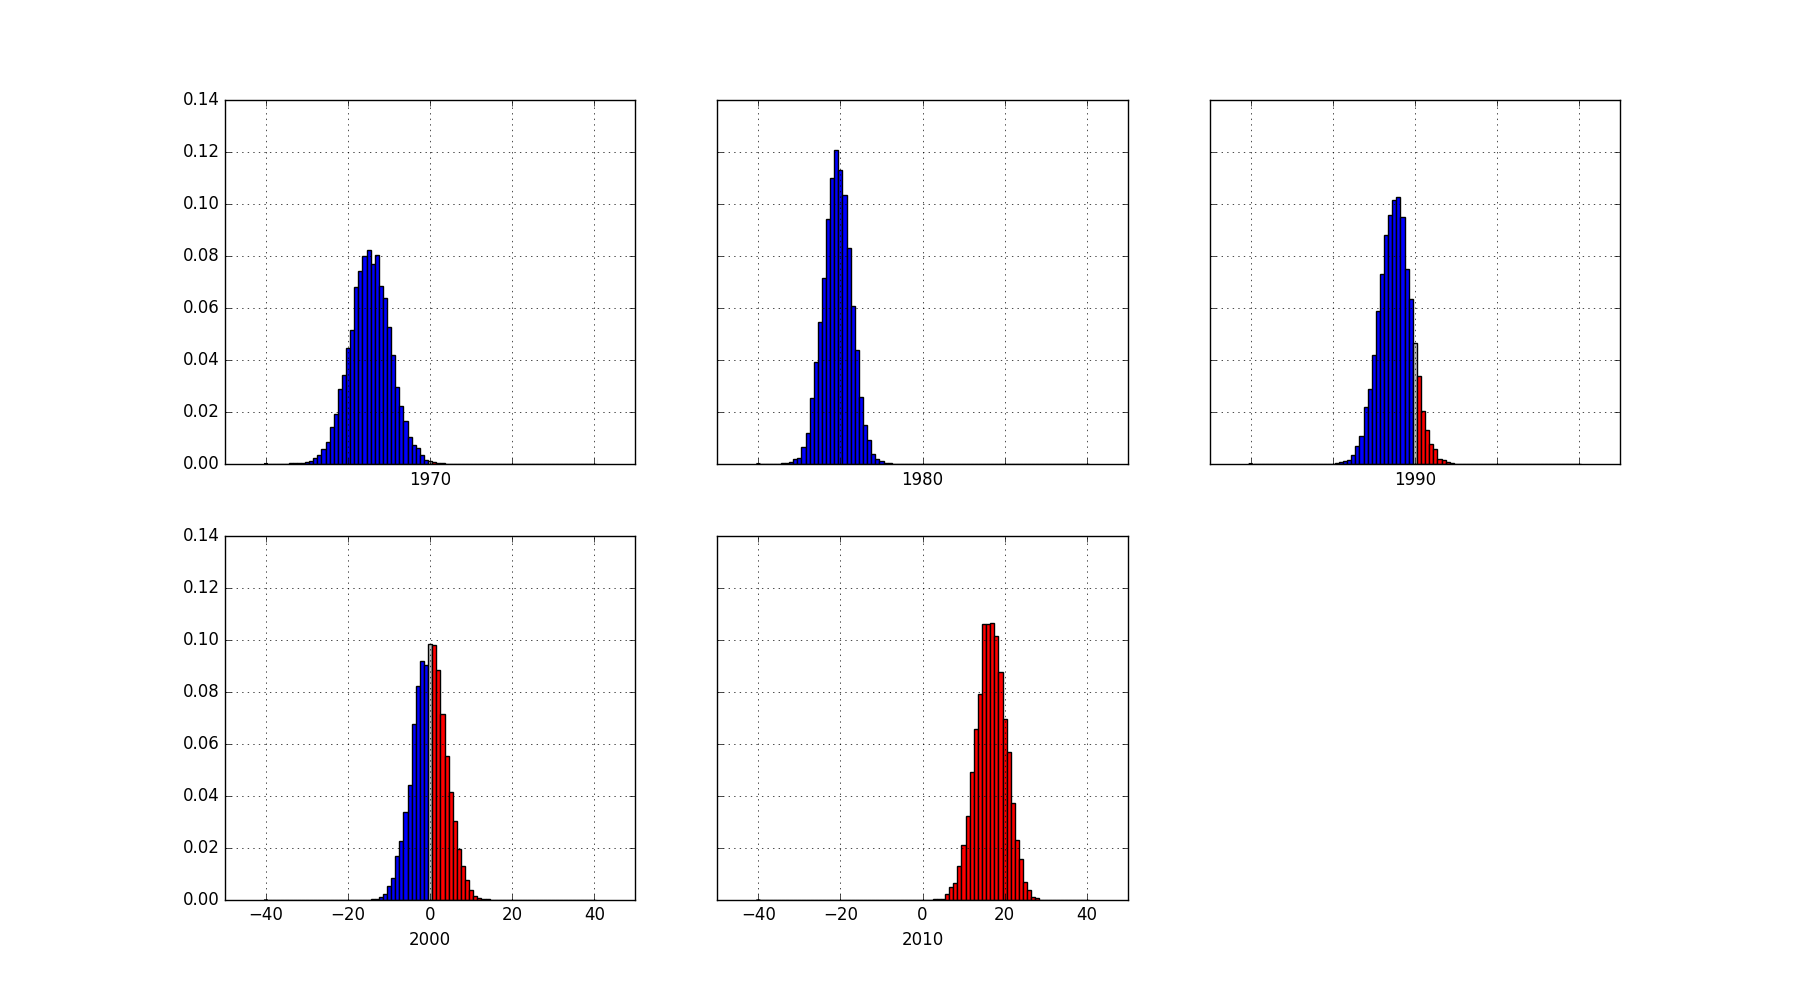
\includegraphics[scale=0.8]{../Figures/ExpectedAsymmetry/netAsymHist.png}
        \caption{Net national asymmetry based on 10,000 simulations}\label{fig:NetAsymHist}
    \end{center}
\end{figure}

The results for the 2010s showing significant Republican gerrymandering are consistent with the well known REDMAP program, where Republicans lead a highly successful effort to gain control of several state houses in advance of the 2010 redistricting.
For earlier cycles, we observe qualitative agreement with a recent study covering the same time period \cite{Wang_2017_} in terms of which party benefited on net from gerrymandering.
Quantitatively, we observe some disagreement in terms of the magnitude of gerrymandering, with the present approach attributing more seats to redistricting bias.
This can be explained by differences in the analysis methodology.
The simulation technique employed in \cite{Wang_2017_} draws a 'fantasy' delegation from national voting results in order to determine if a party is winning seats excessively relative to its vote share\cite{Wang__}.
National voting results are used as a baseline, but this baseline itself will tend to change over time and may contain substantial bias, in which case only large gerrymanders will be successfully identified. 
Since the fantasy delegation technique draws a delegation from existing election results, the likelihood of a highly disproportionate outcome depends on the probability mass in the efficient win region for the party and cycle in question.
To verify this explanation for the differences arising from methodology, consider figure \ref{fig:meanHist}, which shows histograms of the average partisanship in each district and cycle.
There are differences from cycle to cycle in the probability mass in efficient win regions for each party, which arise from a number of causes including changes in redistricting bias.
In contrast, the present approach does not use a national baseline, and instead uses partisan asymmetry as the baseline to judge the effects of gerrymandering.
\begin{figure}[htb!]
    \begin{center}
        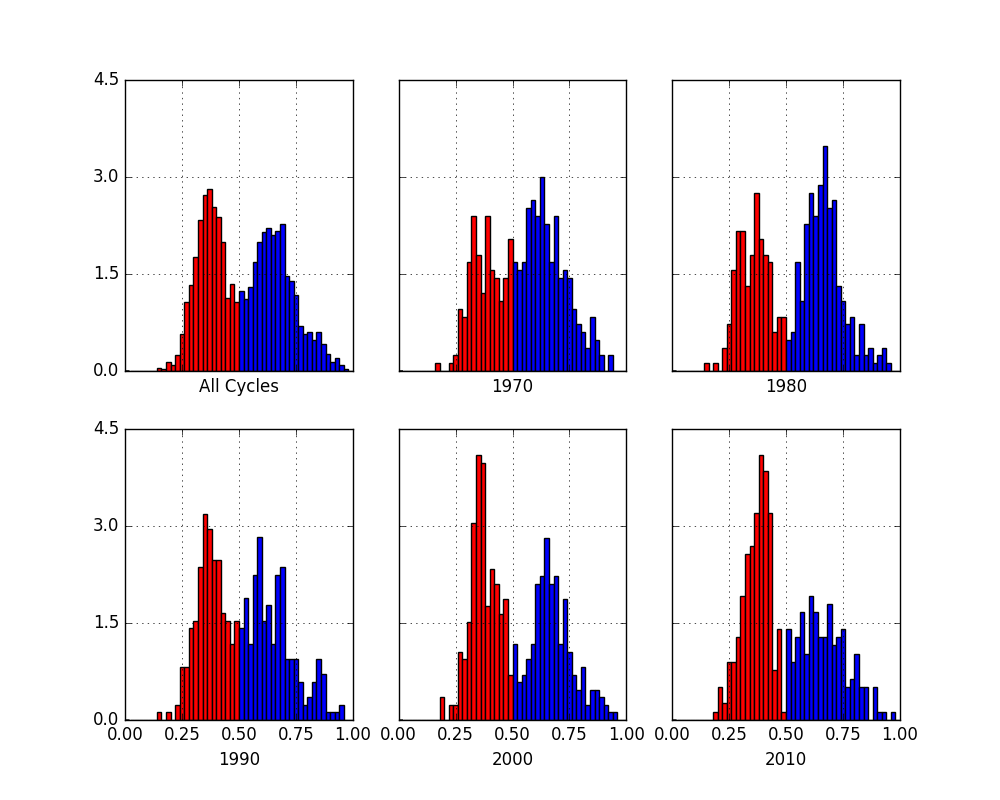
\includegraphics[scale=0.8]{../Figures/HistoricAsymmetry/MeanHist.png}
        \caption{Distribution of mean district partisanship for each cycle}\label{fig:meanHist}
    \end{center}
\end{figure}

Differences in methodology aside, the result that the expected asymmetry favoring Democrats in the 80's is larger than that favoring Republicans in the 2010 cycle is surprising.
In the 2010 cycle, Republicans had the advantages of sophisticated redistricting algorithms, a high degree of geographic polarization, and low variability in voter preferences.
These factors enable effective gerrymandering and would not have been available to redistricters in the 80's.
On the other hand, Democrats controlled a significant number of states in the 80's and the national level of Democratic partisanship in congressional elections was fairly high, while it is closer to even in the 2010 cycle.
Compared to Republicans in the 2010 cycle, Democrats in the 80's obtained seats due to small levels of bias in a number of states, and additionally obtained significant numbers of seats in larger states like California and Texas.
Figure \ref{fig:80vs10} compares the simulated asymmetry distributions for California and Texas in the 80's and for Pennsylvania and North Carolina in the 2010's.
We can see that the variability of the asymmetry in Texas and California was higher than that of Pennsylvania and North Carolina.
It is also worth noting that the number of seats available in these states in the cycles under consideration.
In the 80's Texas has 24 seats and  California had 43, while in the in the 2010's, Pennsylvania had 18 seats and North Carolina had 13.
More district lines offers more opportunities for parties to manipulate redistricting to obtain a partisan advantage, and as a fraction of available seats, the gerrymanders in Pennsylvania and North Carolina are truly remarkable.
This is consistent with the fact that conditions and technology to produce highly stable gerrymanders would exist to a greater degree in the 2010s than in the 1980s.

\begin{figure}[htb!]
    \begin{center}
        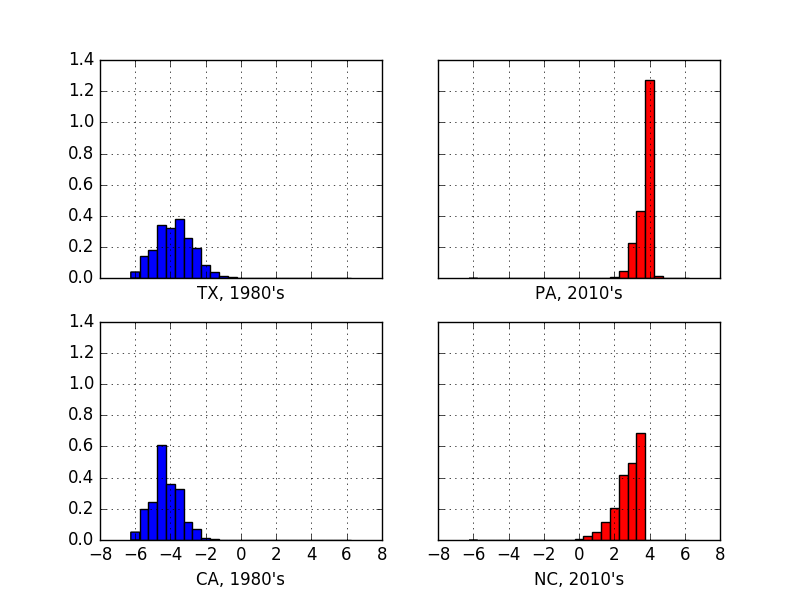
\includegraphics[scale=0.8]{../Figures/ExpectedAsymmetry/80vs10.png}
        \caption{Histograms of the simulated asymmetries in Texas and California in the 1980's, and Pennsylvania and North Carolina in the 2010s}\label{fig:80vs10}
    \end{center}
\end{figure}

Net zero gerrymandering is preferable to a distorted congress, but net zero gerrymandering may still result in the congressional delegations of individual states being highly distorted.
We would therefore also like to examine the total asymmetry, or the sum of asymmetries in all states without regard to which party the asymmetry favors.
This tells us to what extent redistricting is being used to control election outcomes nationally.
This is plotted for each election cycle in \ref{fig:totalAsym}, where we observe that the total asymmetry has held fairly constant over each cycle.
Since there is a fixed number of seats available, every seat of partisan bias that redistrictors secure by gerrymandering is an equal amount of representation taken away from voters.
In other words, the relationship between voter representation and partisan bias resulting from redistricting is that of a zero-sum game: what one side gains, the other side loses.
Regardless of which party benefited from bias on balance, bias in redistricting appears to have affected the representation of millions of voters, for every congressional election since 1972.
\begin{figure}[htb!]
    \begin{center}
        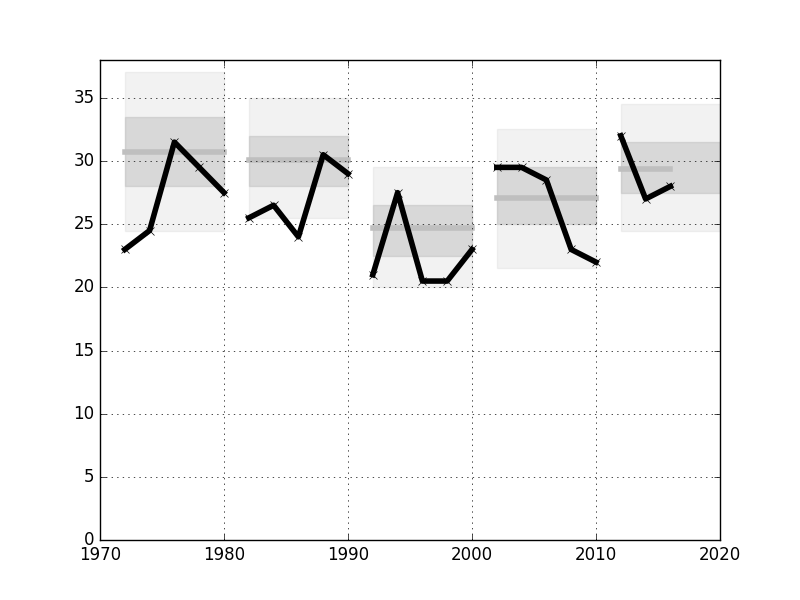
\includegraphics[scale=0.8]{../Figures/ExpectedAsymmetry/totalAsym.png}
        \caption{Total national asymmetry based on 10,000 simulations}\label{fig:totalAsym}
    \end{center}
\end{figure}

While the total national asymmetry has held roughly constant over time, that is not to say that gerrymandering practices have held constant.
To the contrary, some aspects of the 2010 redistricting cycle are quite unprecedented.
Simultaneously, asymmetry has reduced in some states (at least in part due to redistricting reforms enacted in some of those states), while asymmetry has exploded in others.
States known to have been targeted by the REDMAP program are gerrymandered very aggressively in terms of the number of seats available and the level of partisanship in those states.
We can visualize how extreme the most aggressive gerrymanders are in each cycle are by sorting the expected asymmetry (as a percentage of available seats) in descending order for each state.
States with fewer than five seats are excluded since small asymmetries result as very large percentages.
This is shown in figure \ref{fig:asymRank}, where the 2010 cycle stands out as having three states with expected asymmetries that exceeded anything seen previously: Pennsylvania (18.7\%), North Carolina (17.9\%), and Georgia (16.2\%)
Following these are Virginia (12.1\%), Michigan (11.2\%), Ohio (11.0\%), and Wisconsin (9.83\%), which each have large asymmetries by historical standards.
All of these states showed a sudden increase in asymmetry in favor of Republicans after the 2010 redistricting, see table \ref{tab:Asym2000to2010} and figure \ref{fig:Asym2000to2010}. 
In contrast, California and New York had substantial asymmetries favoring Democrats in the 2000 cycle, and while they still show asymmetries favoring Democrats in the 2010 cycle, the magnitude of the asymmetry has decreased.
Previous cycles may have had moderate asymmetries in a larger number of states, but in terms of extreme gerrymandering, there has been no time since the Supreme Court ruled in \emph{Reynold v. Sims} (1964) that congressional districts must have roughly equal population, that is comparable to the 2010 cycle.

\begin{figure}[htb!]
    \begin{center}
        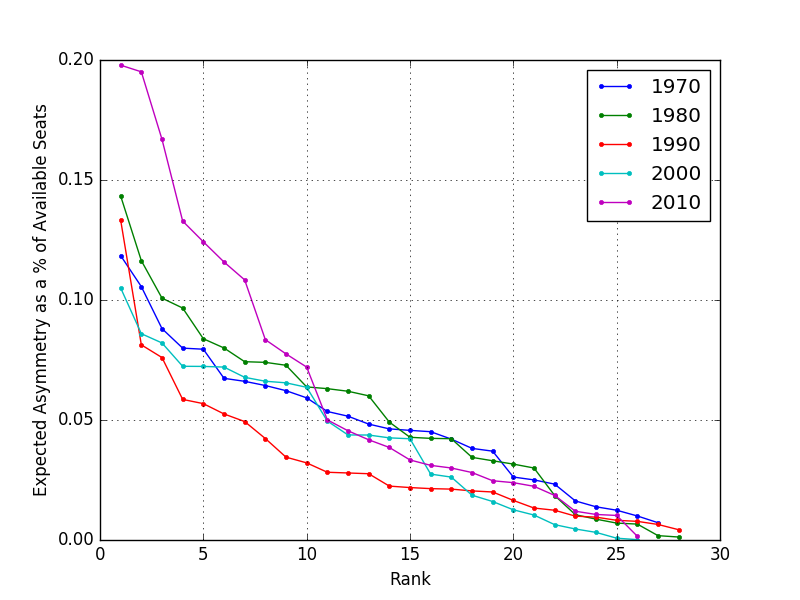
\includegraphics[scale=0.8]{../Figures/ExpectedAsymmetry/asymRank.png}
        \caption{Expected asymmetry as a percentage of seats ranked in descending order for each redistricting cycle}\label{fig:asymRank}
    \end{center}
\end{figure}

\begin{table}[htb!]
\centering
\caption{Change in Expected Specific Asymmetry from 2000 to 2010 for states with large asymmetries in 2010 \label{tab:Asym2000to2010}}
\begin{tabular}{|l|l|l|l|}
\hline
State & Expected Specific     & Expected Specific & Net Change\\
      & Asymmetry, 2000 Cycle & Asymmetry, 2010 Cycle & \\
\hline
\hline
Pennsylvania & R 6.48\% & R 18.70\% & R 12.22\\
\hline
North Carolina & D 4.56\% & R 17.94\% & R 22.51\\
\hline
Georgia & R 3.74\% & R 16.22\% & R 12.48\\
\hline
Virginia & R 6.86\% & R 12.06\% & R 5.20\\
\hline
Michigan & R 6.53\% & R 11.63\% & R 5.10\\
\hline
Ohio & R 7.72\% & R 10.82\% & R 3.10\\
\hline
Wisconsin & D 2.01\% & R 9.90\% & R 11.91\\
\hline
California & D 8.48\% & D 2.17\% & R 6.31\\
\hline
New York & D 7.52\% & D 3.49\% & R 4.04\\
\hline
Illinois & R 0.83\% & D 2.96\% & D 3.79\\
\hline
\end{tabular}
\end{table}

\begin{figure}[htb!]
    \begin{center}
        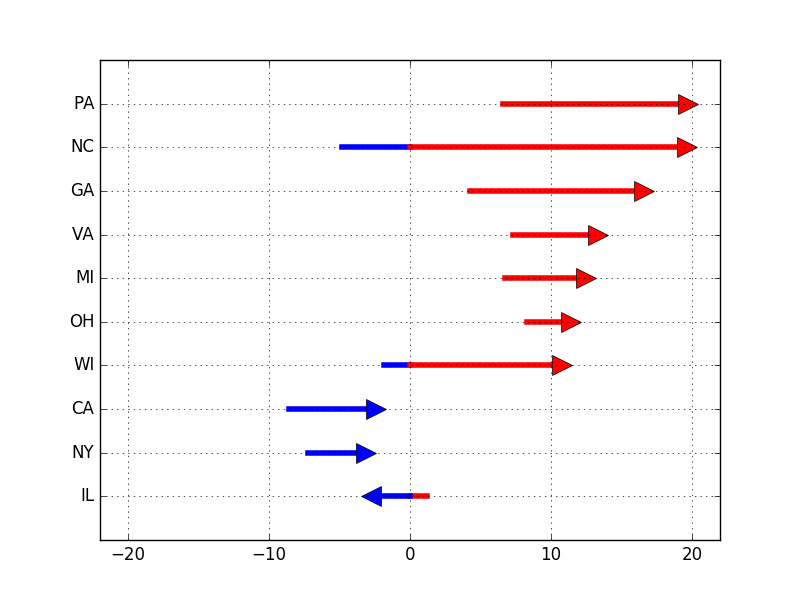
\includegraphics[scale=0.8]{../Figures/ExpectedAsymmetry/diff2000to2010.png}
        \caption{Changes in the expected specific asymmetry from the 2000 redistricting cycle to the 2010 cycle. The arrow indicates the direction of the change in asymmetry.}\label{fig:Asym2000to2010}
    \end{center}
\end{figure}



\section{Partisan Bias in the Wisconsin State Assembly, post 2010 census\label{sec:Wis}}

\begin{figure}[htb!]
    \begin{center}
        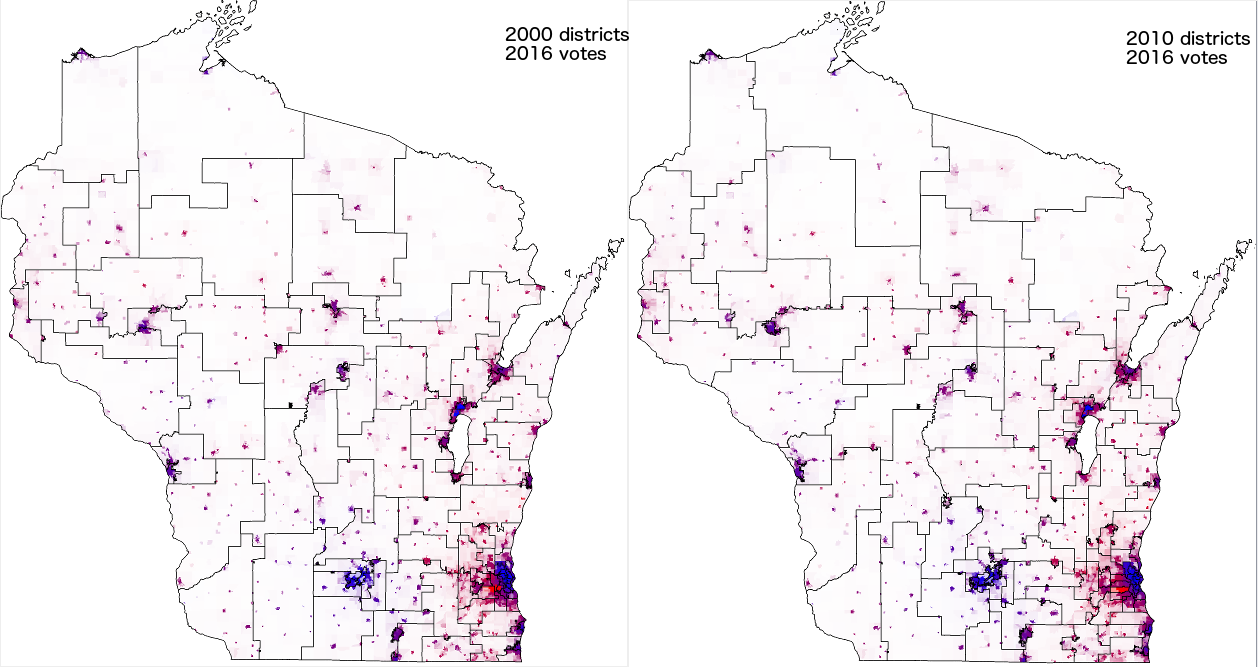
\includegraphics[scale=0.35]{../Figures/WI_compared/precincts_pop_combined.png}
        \caption{2016 Assembly election results by precinct, projected onto Assembly districts before and after Act 43. Left: 2000 cycle districts, Right: 2010 cycle districts}\label{fig:MapsWI}
    \end{center}
\end{figure}

The Wisconsin state assembly districts are the subject of \emph{Whitford v. Gil}, where a federal court has ruled that the redistricting plan is an unconstitutional gerrymander.
The plaintiffs in \emph{Whitford} relied on the efficiency gap to demonstrate bias, while here we apply the expected specific asymmetry.
Some have alleged that the bias in the Wisconsin map is merely the product of changes in voter sentiment and/or political geography.
The argument that there is a natural packing of Democratic voters in urban areas is stated in the Amicus Brief filed by the Republican National Committee and the National Republican Congressional Committee.
The tendency of Democratic voters to cluster in urban areas is well known, but no proof was offered to suggest that the electoral advantage given to Republicans in the Act 43 map was merely the result of this effect an not of deliberate gerrymandering.
The RNC and NRCC brief cited the studies of Chen and coworkers in support of the notion that gerrymandering can occur unintentionally due to population clustering \cite{Chen_2015_10.1089/elj.2015.0317,Chen_2016_10.1016/j.electstud.2016.06.014} among others, although interestingly a recent study of the Act 43 map by Chen \cite{Chen_2017_} using the same analysis technique from these previous studies concluded the following: \emph{Act 43 not only created an extremely biased Assembly plan with an efficiency gap far outside of any gap observed in 200 simulations, the enacted plan achieved this partisan outcome at the expense of traditional districting principles, splitting apart far more counties and municipalities than were necessary.}
The fact that the Act 43 map does not attempt to preserve existing political boundaries directly undercuts the argument that the bias in the map arises from natural political geography.
In what follows, we employ a different analysis methodology and find that the Act 43 map leads to an increase in seats won by Republican candidates by increasing the partisan asymmetry in their favor relative to the previous map.
This is further evidence that the bias in the Act 43 map reflects the deliberate intentions of the redistricters, and simply can not be explained by political geography alone.

To compare how much of the observed partisan asymmetry in 2010-cycle Wisconsin State Assembly districts was the result of changes in district designs versus changes in voter sentiment, we projected actual election results onto both the current Assembly districts, and Assembly districts from the previous redistricting cycle, as shown in figure \ref{fig:MapsWI}.
This allows us to analyze the effects of changes in voter sentiments and redistricting separately.

For this analysis we used official districting plans for the 2000 and 2010 census cycles, and actual vote counts from the 2006, 2008, 2010, 2012, 2014, and 2016 assembly elections, at precinct-level resolution, imputing uncontested elections with partisan swing matched presidential election results when available, and partisan swing matched federal congress election results when not.
By "partisan swing matched" we mean that the Republican vote counts in all districts are multiplied by a constant factor so that the total vote count matches that for the assembly elections, for the subset of districts in which both elections were contested, and the same is done for the Democratic vote counts.
Then election data for 2006, 2008, and 2010 were cross-aggregated at census block resolution to the 2010-cycle districts, and election data for 2012, 2014, and 2016 were cross-aggregated at census block resolution to the 2000-cycle districts. 
Since the same exact elections are used in both the 2000 districts analysis and 2010 districts analysis, \emph{all} differences in the results are the consequence of the redistricting scheme used, and conversely, changes in voter sentiment have exactly \emph{zero} contribution to the difference.

If the 2000 census cycle districts show a partisan asymmetry much lower than the 2010 cycle, then we would know that natural "political geography" -- the tendency of Democratic voters to be clustered in cities -- can be immediately ruled out as a significant factor in the partisan asymmetry inherent in 2010 cycle Wisconsin Assembly districts, since any contributions from political geography would be present in \emph{both} districting schemes.
However if they are not substantially different, this would not demonstrate that political geography was a significant contribution, because they both could be artificially gerrymandered on top of any unintentional gerrymandering due to political geography.
In this case, further analysis would be required to separate the effects of unintentional bias caused by political geography and deliberate bias caused by gerrymandering.

\subsection{Observed partisan asymmetries in past elections}

\begin{figure}[htb!]
    \begin{center}
        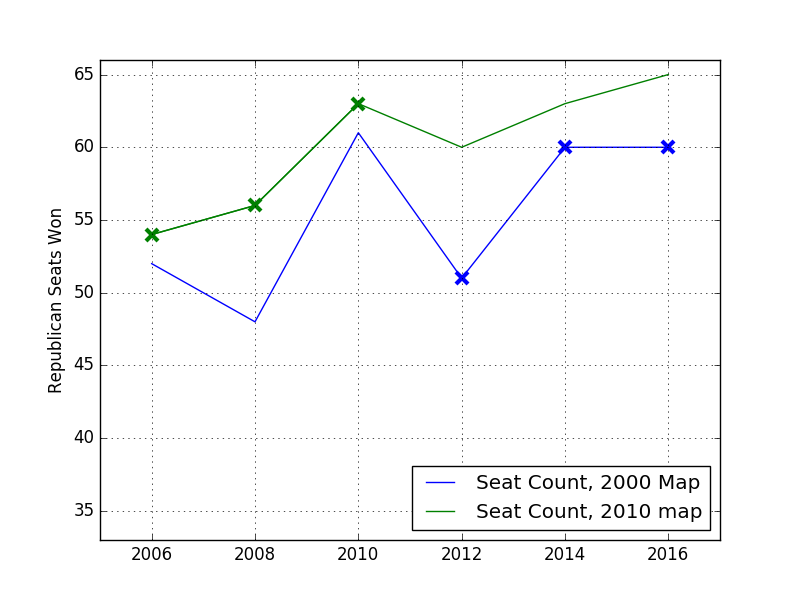
\includegraphics[scale=0.85]{../Figures/WI2010/WI_2000_2010_seats.png}
        \caption{Republican Seat Counts in Assembly elections, using 2000 cycle districts vs 2010 cycle districts. The X's indicate that a result has been cross aggregated, meaning results were computed on a different district map than the one that actually existed at the time of the election.}\label{fig:Seats20002010}
    \end{center}
\end{figure}

\begin{figure}[htb!]
    \begin{center}
        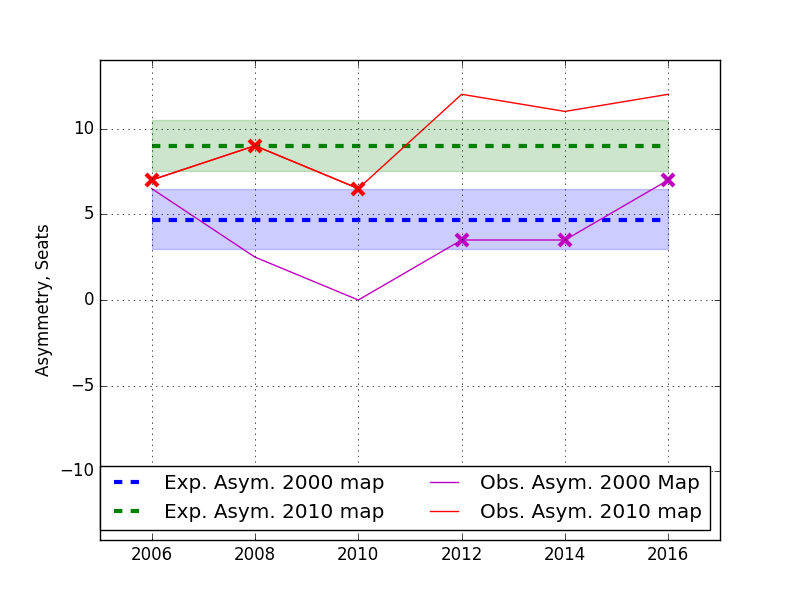
\includegraphics[scale=0.85]{../Figures/WI2010/WI_2000_2010.png}
        \caption{Historical asymmetry in Assembly elections, using 2000 cycle districts vs 2010 cycle districts. The X's indicate that a result has been cross aggregated, meaning results were computed on a different district map than the one that actually existed at the time of the election.  The dashed lines represent the statistical expectations, and the shaded areas represent the 50\% confidence intervals.}\label{fig:Asym20002010}
    \end{center}
\end{figure}

After imputing uncontested elections and projecting onto the two different districting schemes, we counted up the wins and computed the specific asymmetry for each election on each map.
The seat counts are shown in figure \ref{fig:Seats20002010}, and the specific asymmetry is shown in figure \ref{fig:Asym20002010}.  They are also tabulated in table \ref{tab:seats}.
The horizontal lines and shaded regions represent the statistical expectation and 50\% confidence intervals, respectively.

The charts show a clear and stable separation between both seat counts and partisan asymmetry between 2000 districts and 2010 districts.
They both go up and down largely in parallel, responding about the same to changes in voter sentiment.
This tells us that in the 2012, 2014, and 2016 elections, the new districts led to an increase in Republican representation over what the old districts would have produced.
Furthermore, were the new districts used in the 2000 redistricting cycle, that would have produced about the same increase in Republican representation for the 2006, 2008, and 2010 elections.

\begin{table}[htb!]
\centering
\caption{Summary of the differences in seat counts and asymmetries for elections on the two legislative maps \label{tab:seats}}
\begin{tabular}{|l|l|l|l|}
\hline
Election Year & Rep. Seats, 2000 Map & Rep. Seats, 2010 Map & Net Change in Seats\\
\hline
\hline
2006 & 52 & 54 & R + 2\\
\hline
2008 & 48 & 56 & R + 8\\
\hline
2010 & 61 & 63 & R + 2\\
\hline
2012 & 51 & 60 & R + 9\\
\hline
2014 & 60 & 63 & R + 3\\
\hline
2016 & 60 & 65 & R + 5\\
\hline
\hline
Election Year & Asymmetry, 2000 Map & Asymmetry, 2010 Map & Net Change in Asymmetry\\
\hline
\hline
2006 & 6.5 & 7.0 & R + 0.5\\
\hline
2008 & 2.5 & 9.0 & R + 6.5\\
\hline
2010 & 0.0 & 6.5 & R + 6.5\\
\hline
2012 & 3.5 & 12.0 & R + 8.5\\
\hline
2014 & 3.5 & 11.0 & R + 7.5\\
\hline
2016 & 7.0 & 12.0 & R + 5.0\\
\hline
\end{tabular}
\end{table}


In figure \ref{fig:Asym20002010diff}, the difference in seats won by Republicans is plotted along with the difference in the expected asymmetries between the two maps.
The increase in seats gained by Republicans in the 2010 map is entirely explained by the increase in asymmetry in the 2010 map.
Therefore the 2010 map leads to greater Republican representation by \emph{structurally disadvantaging Democratic voters}.


\begin{figure}[htb!]
    \begin{center}
        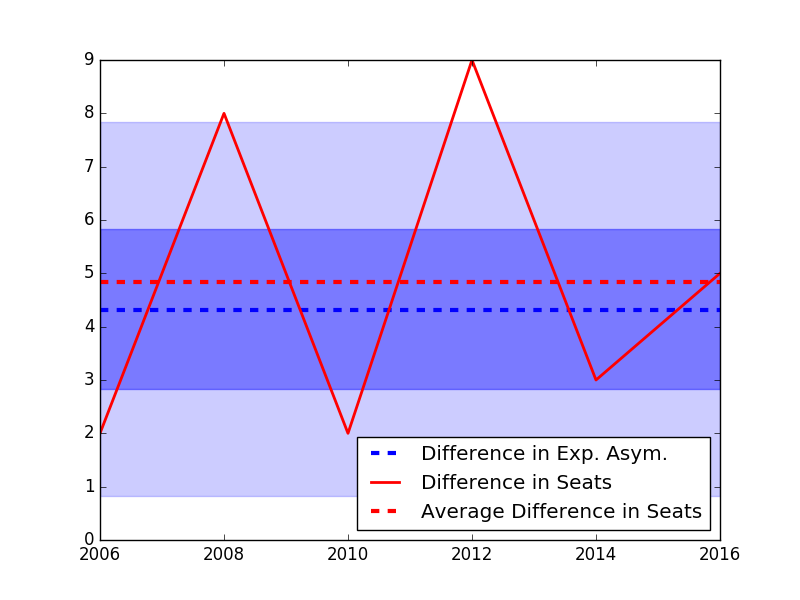
\includegraphics[scale=0.85]{../Figures/WI2010/WI_2000_2010diff.png}
        \caption{Difference in seats won by Republicans in the two maps. The dashed blue line shows the difference in expected asymmetry between the two maps, the blue and light blue shaded regions represent 50\% and 90\% confidence intervals}\label{fig:Asym20002010diff}
    \end{center}
\end{figure}

\begin{figure}[htb!]
    \begin{center}
        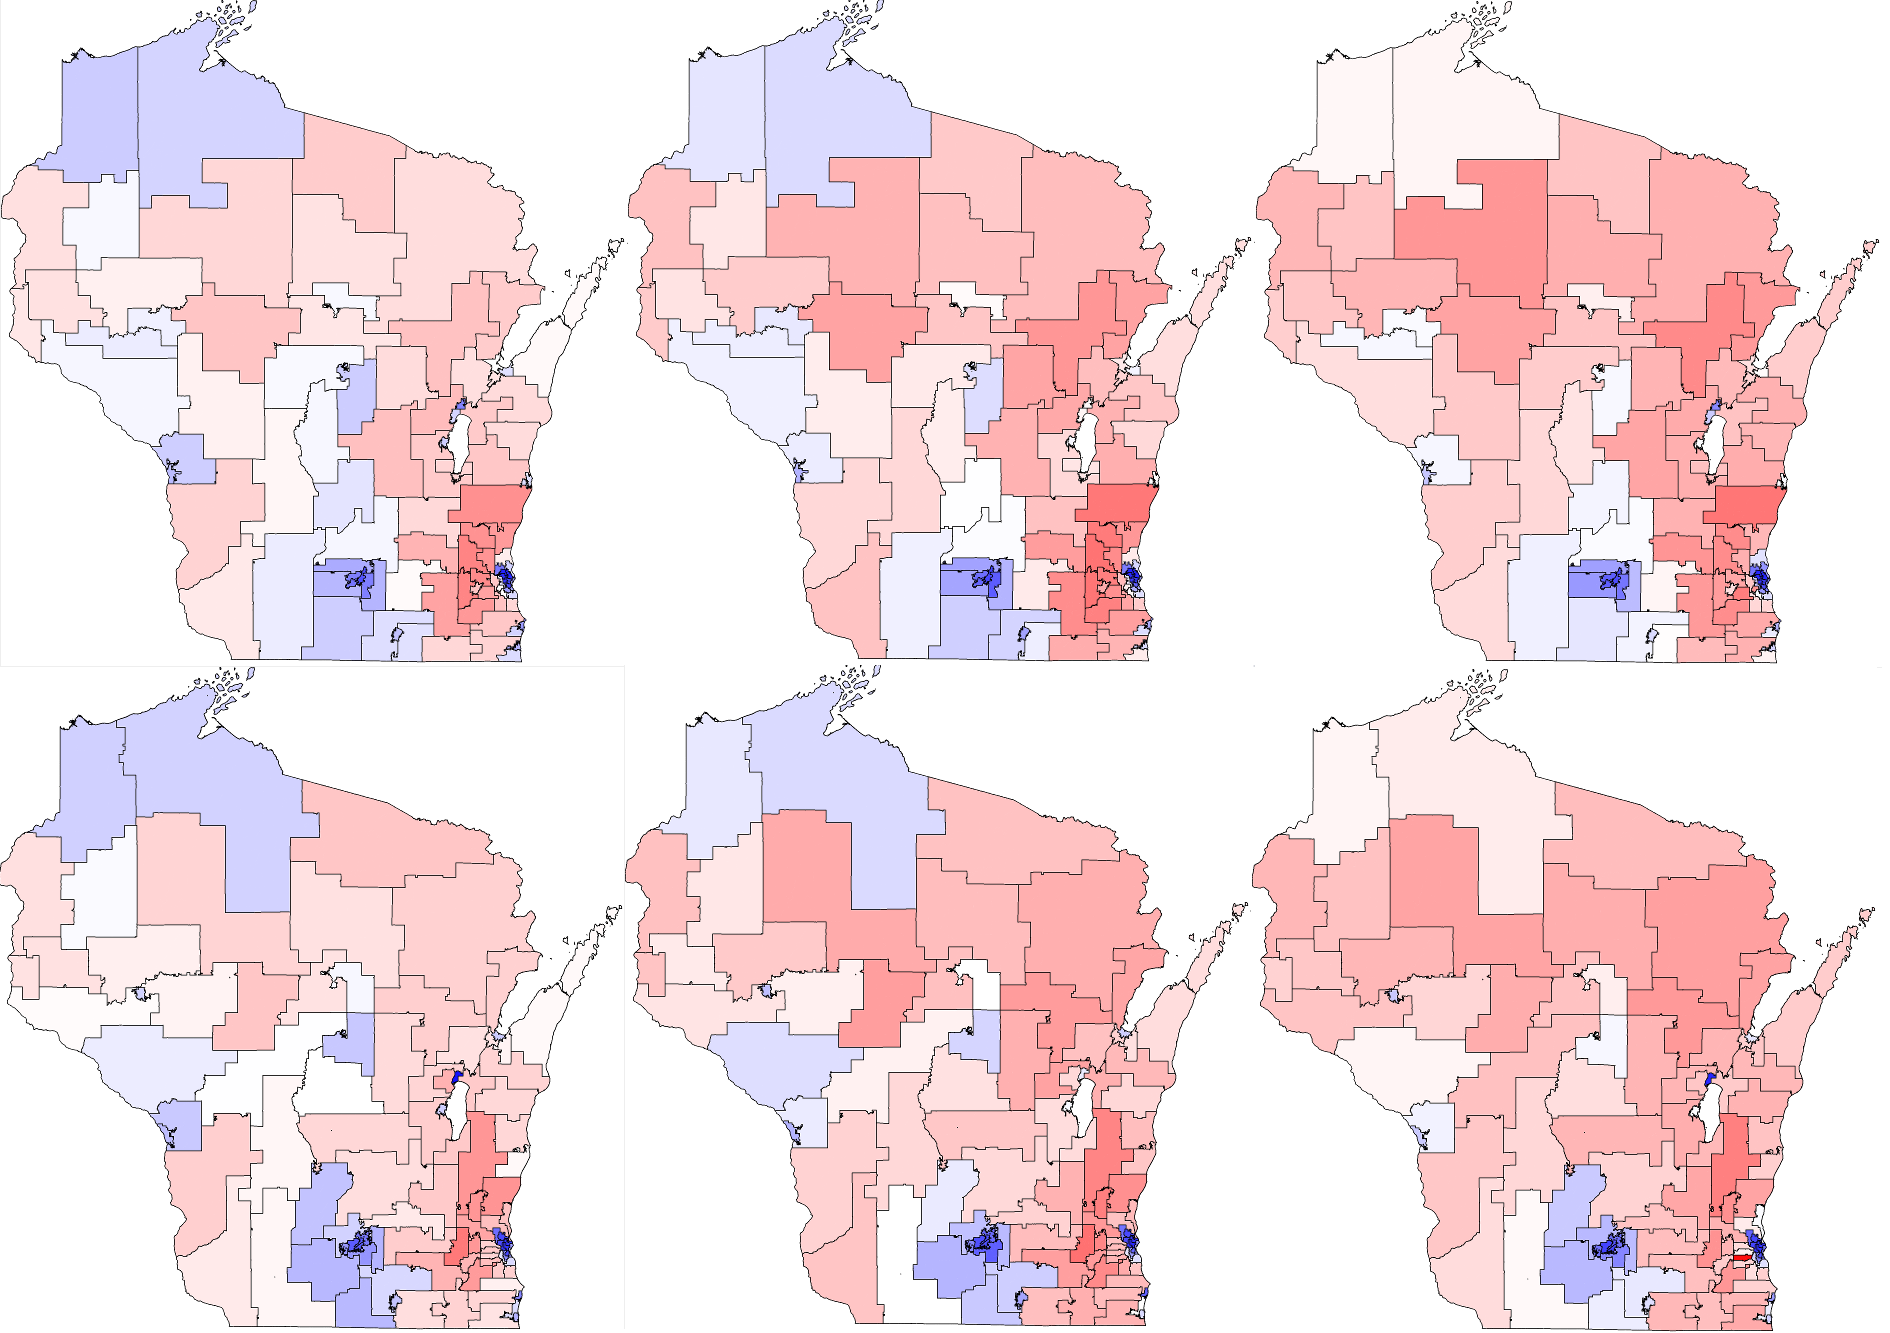
\includegraphics[scale=0.25]{../Figures/WI_compared/3x2.png}
        \caption{Partisan vote packing in Wisconsin Assembly elections. Top: 2000 cycle districts, Bottom: 2010 cycle districts, Left to right: 2012, 2014, and 2016 elections.}\label{fig:DistrictMaps}
    \end{center}
\end{figure}


We can better visualize how the 2010 districts give Republicans more seats than the 2000 districts by coloring in the districts according to the victory margin, and comparing.
Figure \ref{fig:DistrictMaps} shows such a comparison for 2012, 2014, and 2016 elections (left to right).
The two Democratic districts above Lake Winnebago were combined into one, taking a seat away from Democrats.
Democratic voters in Eau Claire once participated in two competitive districts, which would have given Democrats 2 seats with 2000 district lines, but the 2010 district lines wrapped them up in a single safe district, capping the number of elections those voters can swing at 1.
In 2000 districts, Madison is surrounded by several competitive Democratic-leaning districts.
But the 2010 lines packed Democratic voters surrounding Madison into a few safe Democratic districts, flipping the districts those voters came from, which would have been competitive, to Republican.
In Milwaukee, the lines were redrawn to more tightly outline Democratic voters, thus creating a few more districts that Republicans can win in.
Indeed, figure \ref{fig:DistrictMapDelta} shows that by comparing the districting schemes using 2016 votes, it is easy to identify where Republicans picked up 4 seats due to partisan vote packing.

Simultaneously, deeper red districts throughout the state were redrawn to give away some of their Republican voters to nearby competitive districts, reducing the likelihood that a Democratic representative would be elected in the once-competitive districts while still maintaining a safe edge in the originally deeper red district.  
You can see this by noticing the much "flatter" red color in the bottom maps versus the top maps.
It will also be made clear in the next subsection when we examine the statistical properties of the maps more rigorously.
fs
In sum, the changes in the district lines from 2000 districts to 2010 districts consist of decreasing the number of Democratic districts through vote packing, and increasing the number of Republican districts through vote cracking.
Instances of the reverse (packing Republican voters and cracking Democratic districts) are simply not present.
\begin{figure}[htb!]
    \begin{center}
        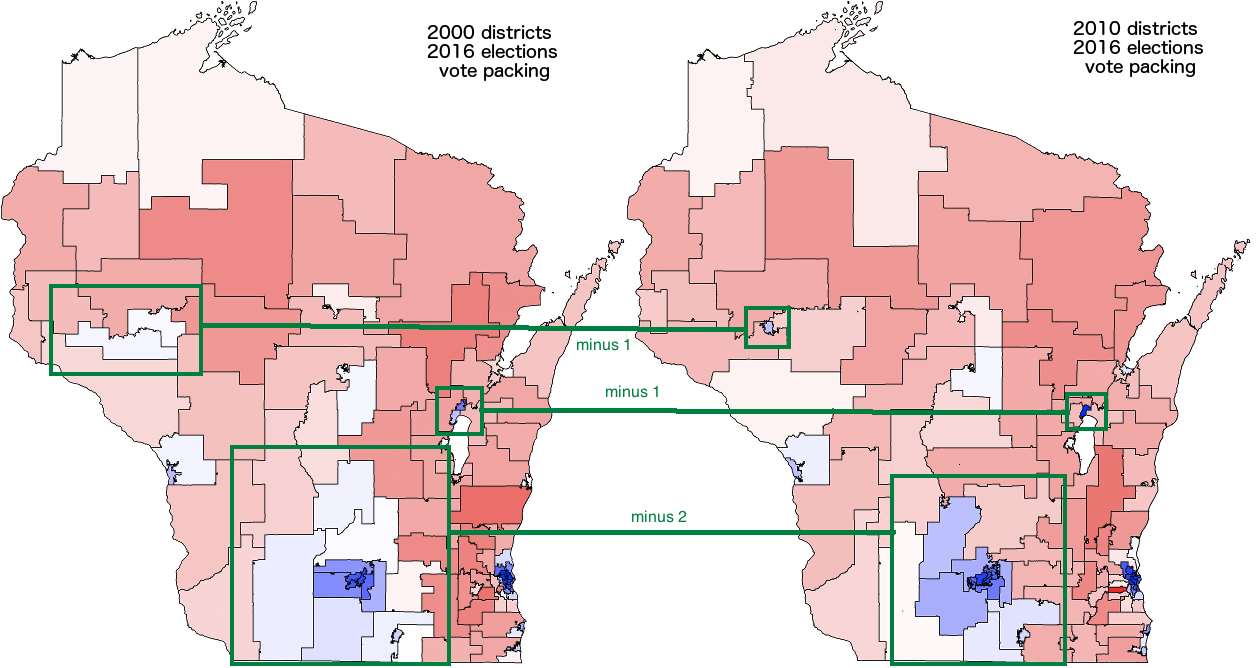
\includegraphics[scale=0.40]{../Figures/WI_compared/districts_compared_deltas.png}
        \caption{Partisan vote packing in Wisconsin Assembly elections, using 2016 election data.  Outlined in green are areas where Republicans packed Democratic votes.}\label{fig:DistrictMapDelta}
    \end{center}
\end{figure}



\subsection{Expected  partisan asymmetries in future elections}

\begin{figure}[htb!]
    \begin{center}
        \includegraphics[scale=0.25]{../Figures/WI_compared/Betas_cropped.png}
        \caption{Beta distributions for Wisconsin 2010-cycle Assembly districts, Top: 2000 cycle districts, Bottom: 2010 cycle districts}\label{fig:BetasWI}
    \end{center}
\end{figure}
 
Figure \ref{fig:BetasWI} shows the beta distributions estimated for each district and the popular vote under the 2000 and 2010 redistricting plans. 
Before evaluating this model with Monte Carlo sampling, we can find some clear signs of pro-Republican gerrymandering just from inspection of these distributions. 
Many Republican-leaning districts are tightly clustered at levels of partisanship that allow Republican candidates to win safely without wasting too many votes, while many Democrat-leaning districts are heavily packed and not competitive.
In the 2010, distributions Republicans-leaning districts are more concentrated around a single point slightly but safely short of competitive, while Democratic-leaning districts that were competitive in the 2000 distributions have been shifted away from the center.
Consequently, in the 2010 distributions, compared to the 2000 distributions, Republicans are expected to gain more seats by smaller margins, while Democrats are expected to gain fewer seats by larger margins.


\subsubsection{Specific partisan asymmetry likelihoods}
 
The results of Monte Carlo integration are shown in figure \ref{fig:LikelihoodsAsymmetry}, as a fraction of total available seats.  
These results were also used to compute the expectations and confidence intervals shown in figures \ref{fig:Asym20002010} and \ref{fig:Asym20002010diff}.
 
\begin{figure}[htb!]
    \begin{center}
        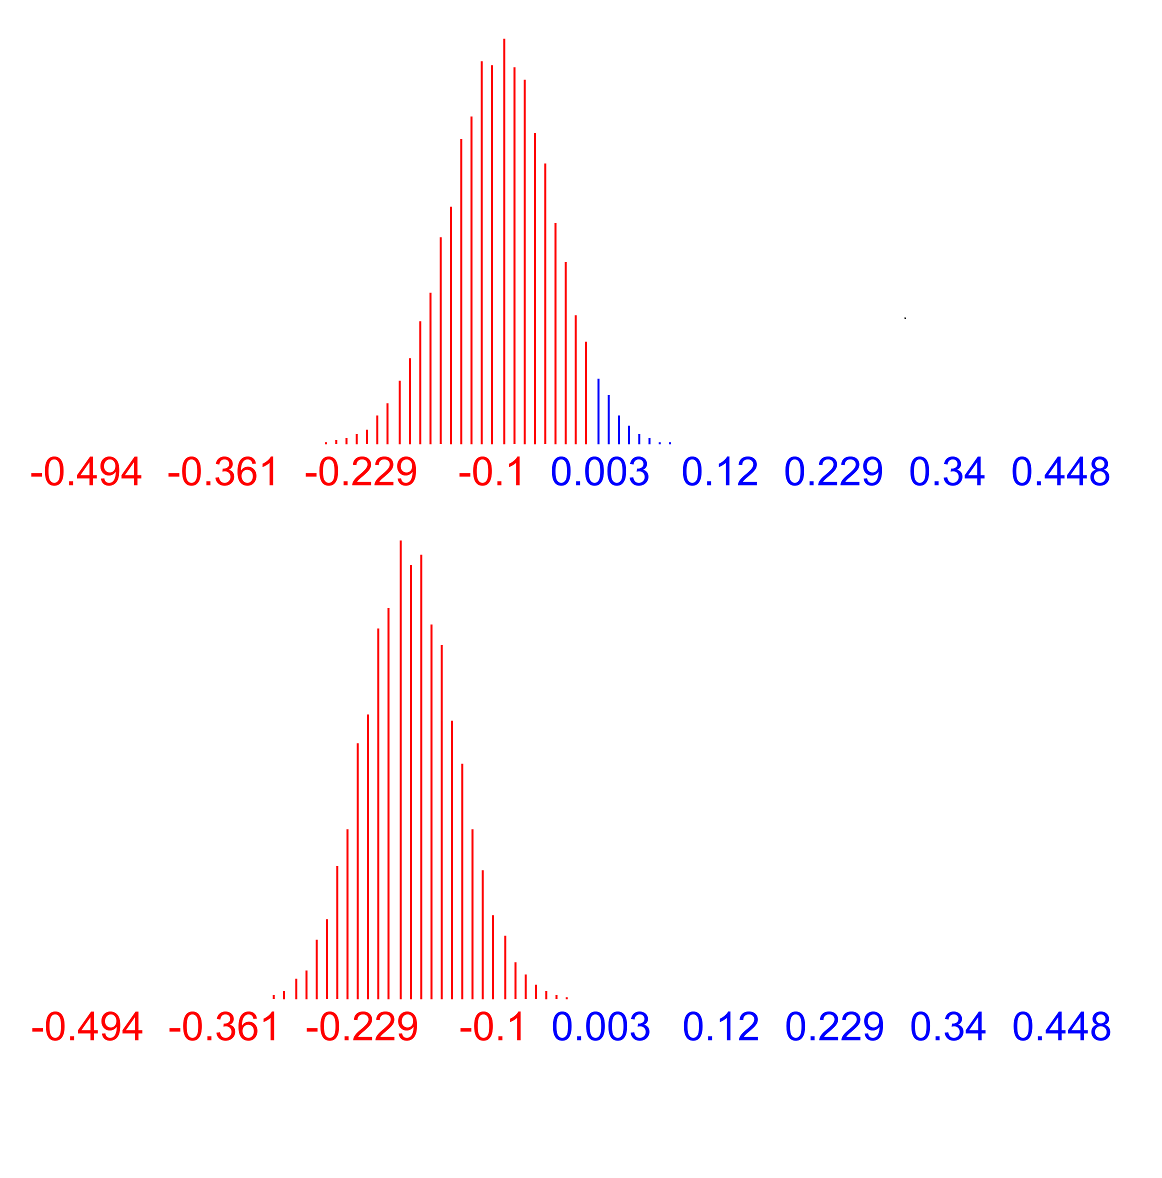
\includegraphics[scale=0.25]{../Figures/WI_compared/asymmetry_cropped.png}
        \caption{Specific asymmetry likelihoods, Top: 2000 cycle districts, Bottom: 2010 cycle districts}\label{fig:LikelihoodsAsymmetry}
    \end{center}
\end{figure}
 
For the 2000 districts, the partisan asymmetry favors Republicans, giving them an average seat boost of 10\% of the available seats beyond what a symmetric seats-votes curve would produce.  
However, there is still a decent likelihood that voter sentiments would change enough that Democrats would get a small boost from seats-votes curve asymmetry.

For the 2010 districts, the partisan asymmetry favors Republicans by twice the amount of the 2000 districts, giving them an average seat boost of 20\% of the available seats beyond what a symmetric seats-votes curve would produce.  
The most likely result in the Wisconsin state assembly might be that Republicans get 6/10ths of the legislative seats, whereas if the popular vote count were reversed, Democrats would get only 4/10th of the legislative seats.  
Remedying this would give Democrats 10\% more seats.  
This means that roughly 10\% of the entire Democratic-voting population of the state of Wisconsin were effectively disenfranchised, in violation of the one person, one vote principle.  
Conversely, 10\% of the Republican-voting population effectively got an extra vote, which is approximately equivalent to 306,000 cases of illegal voting.
This is a very large gerrymander relative to what was found in our examination of U.S. congress.

Unlike the 2000 districts, out of 100,000 samples drawn, \emph{none} of them resulted in specific partisan asymmetry favoring Democrats.  
Since an assembly district election occurs every 2 years, this shows that, without significant changes in geo-spatial demographics, the asymmetric pro-Republican partisan advantage inherent in this redistricting will persist for the next 200,000 years.

\subsubsection{District partisanship histogram}
  
\begin{figure}[htb!]
    \begin{center}
        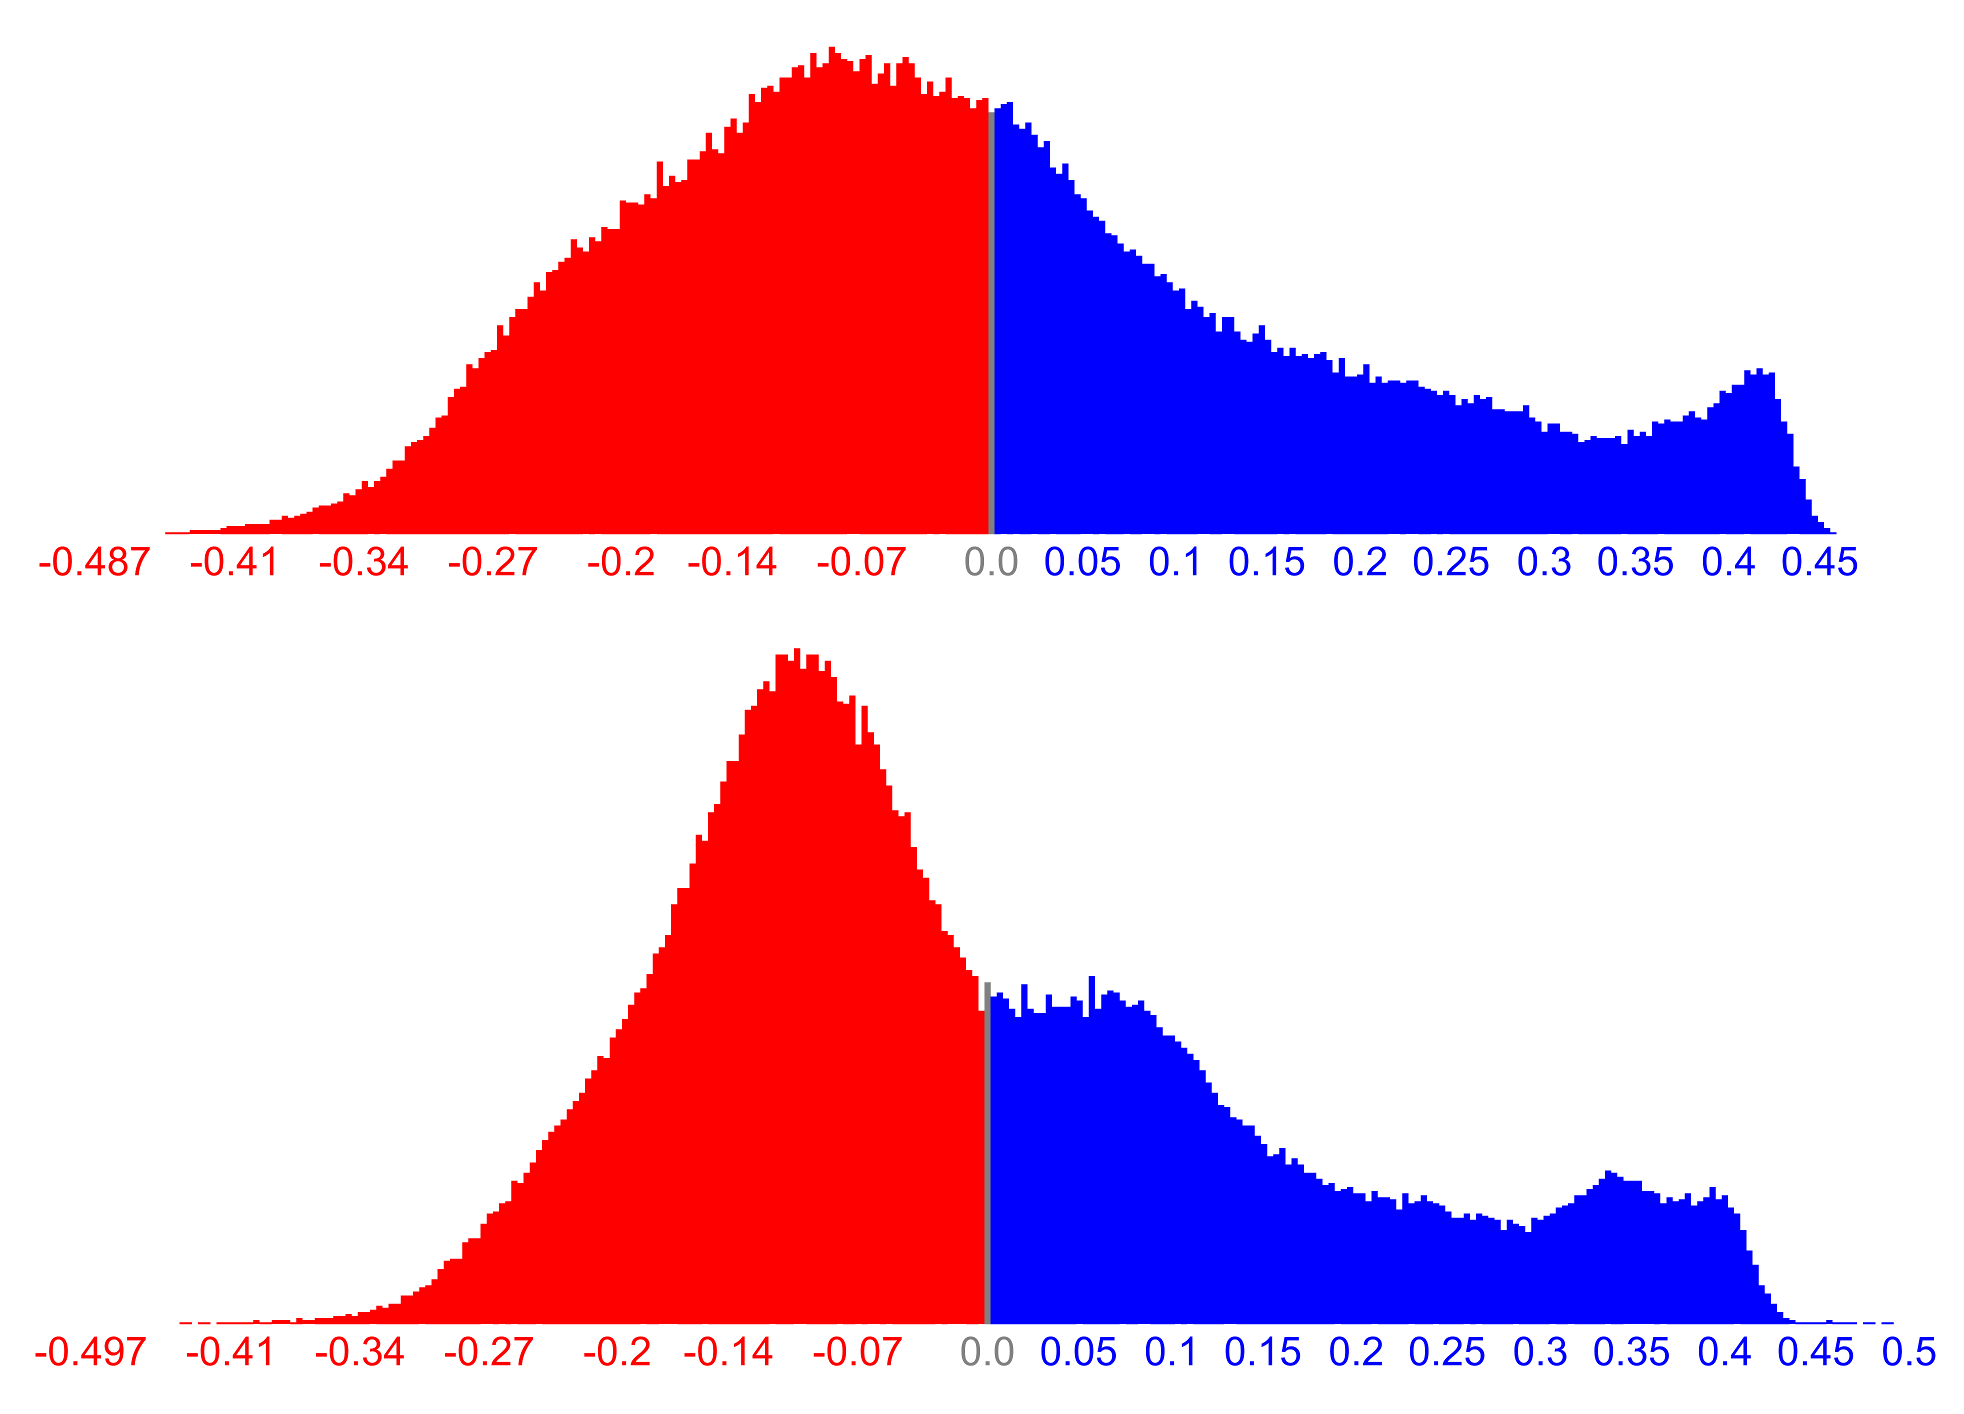
\includegraphics[scale=0.25]{../Figures/WI_compared/district_partisanship_cropped.png}
        \caption{District partisanship likelihoods, Top: 2000 cycle districts, Bottom: 2010 cycle districts}\label{fig:LikelihoodsDistrictPartisanship}
    \end{center}
\end{figure}

Another way we can visualize the partisan asymmetry in the Wisconsin state assembly map is by looking at the histogram of district partisanship.
The same Monte Carlo integration technique we used to compute the expected specific asymmetry can be used to construct the likelihood function for district partisanship over all districts and all possible election outcomes.
In other words, if one were to pick a random district in a random election, this curve shows how likely the vote in that district is to be 25\% Republican vote, a 50-50 split, etc.
 
The curve for the 2000 districts show a smooth peak near 50/50, with a slight skew towards Republicans and a long tail on the Democratic side with a brief peak at the end.  
This shows that Democratic districts were packed, while Republican districts were cracked.

On the other hand the curve for the 2010 districts show a much sharper distinction.
It has a high red peak close to the center but still safely to the side, that already drops off sharply by the time it hits 50/50, and then on the blue side, drops slowly all the way until it gets to a larger bump at the extremely packed end of the scale.
This clearly reveals that Republican candidates in Republican leaning districts have a high likelihood of winning safely but without wasting too many votes, while Democratic candidates in Democratic leaning districts have a high likelihood winning by margins that waste a lot of votes.
You can also see this effect visually on the maps in figure \ref{fig:DistrictMaps}: the red colors are much "flatter" in 2010 districts (bottom) than 2000 districts (top).

\subsubsection{Statewide seat count likelihoods}

\begin{figure}[htb!]
    \begin{center}
        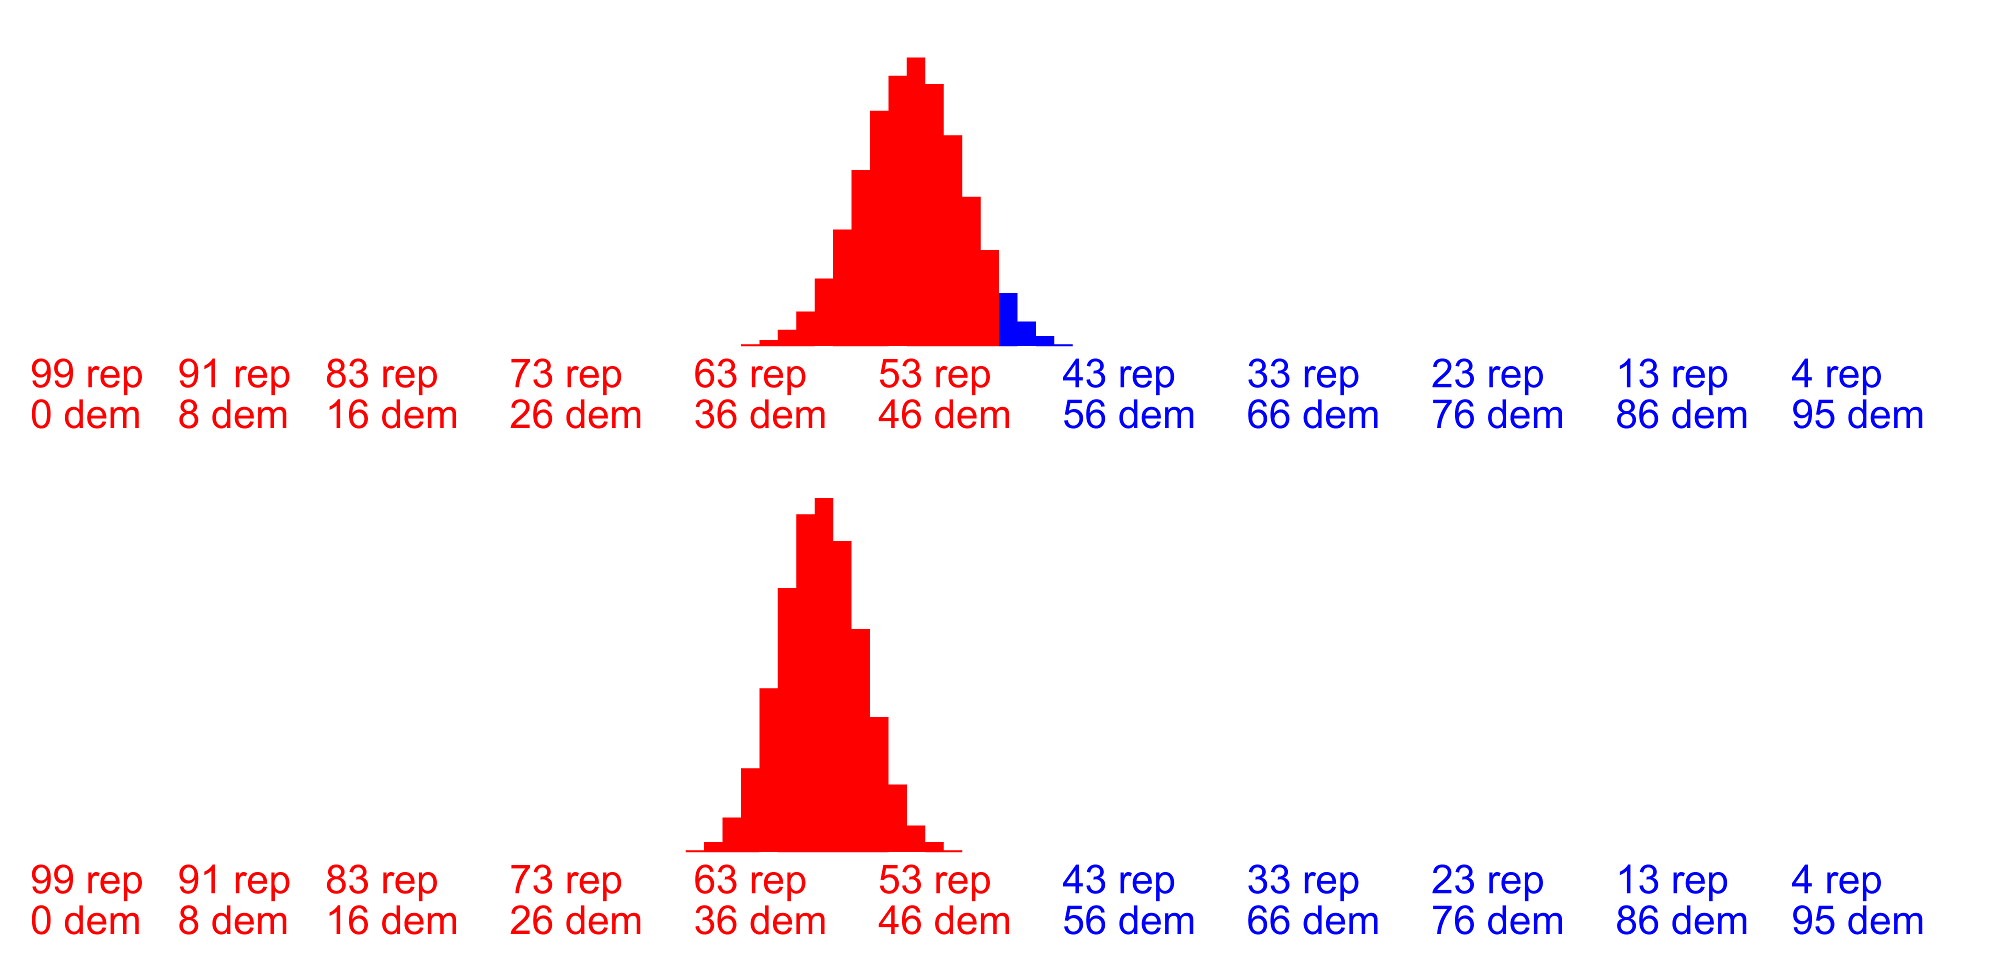
\includegraphics[scale=0.25]{../Figures/WI_compared/seats_cropped.png}
        \caption{Seat count likelihoods, Top: 2000 cycle districts, Bottom: 2010 cycle districts.}\label{fig:LikelihoodsSeatCounts}
    \end{center}
\end{figure}
 
A third way to use the Monte Carlo results to understand asymmetry is to estimate the likelihood of every possible election outcome, district-by-district.
We then accumulate these outcomes on a chart, with the seat count on one axis, and the likelihood on the other.  The results are shown in figure \ref{fig:LikelihoodsSeatCounts}.

In 2000 districts, the expected outcome is for Republicans to win a 54-45 majority of seats, though Democrats still have a decent chance of winning the majority of seats. 
In 2010 districts, Republican's expected lead grows by an additional 10 seats to 59-40. 
Despite being favored by roughly half the voters, Democrats have no chance at all to win a majority of seats even in the most eccentric swings of voter sentiment.
Out of 100,000 samples, Democrats rarely even get 45 of the seats, which was their average under the 2000 districting scheme.

\subsection{Discussion}

Measured by partisan asymmetry, both expected and observed, there was substantial gerrymandering in favor of Republicans in the 2000 cycle maps.
This asymmetry leads to about 4 extra Republican seats beyond what would be allocated if the seats-votes curve was symmetric.
The current method does not distinguish what part of this gerrymandering was deliberate and what part unintentional, though regardless of the proportion, it is trivial to generate a map without this asymmetry by using one of many well-known optimization algorithms.

If we disregard data that was not available when the 2010 cycle districts were drawn, and use only data from the 2006, 2008, and 2010 elections, we see that with the new redistricting lines, Republicans are expected to gain an additional 4 assembly seats (an 8 seat swing), beyond what the previous (2000 cycle) redistricting lines would have given them.
Furthermore, this is in addition to the partisan asymmetry already present in the 2000 cycle maps, bringing the expected total seat difference gained over Democrats through partisan asymmetry to 18.

The fact that the 2010 cycle maps have double the partisan asymmetry as the 2000 maps demonstrates that regardless of what part of the gerrymandering in the 2000 cycle maps was deliberate, \emph{at least} half of the gerrymandering in the 2010 cycle maps was deliberate.
In any case, a map optimized by a computer algorithm to maximize partisan symmetry could remove almost all of the deliberate gerrymandering, and at least some of the unintentional gerrymandering.

From these comparisons, it is clear that the specific partisan asymmetry present in the 2010 cycle districts is \emph{not} present in the 2000 cycle districts, even when using vote count data from the exact same elections.  Therefore:
\begin{itemize}

\item The difference between the two schemes is a stable 10\% gain in the Republican seat margin over Democrats.
Since the same exact voter sentiments were used in both analyses, this difference in partisan asymmetry simply cannot be a consequence of changes in voter sentiment.  
Since the only thing that we changed was the districting scheme, all observed differences in partisan asymmetry are purely the result of changing the districting scheme and reflect the choices made by the redistricters and do not reflect changes in political geography.
\item Claims that the election results it produced are similiar to those under the previous districts are categorically false.
\item In order to claim that natural political geography was a significant factor in the 2010 cycle district, we would expect to see the exact same asymmetries in the 2000 districts.
To the contrary, partisan asymmetry in 2010 districts is double that of 2000 districts, even after compensating for observed and potential changes in voter sentiment.
\item Claims that the observed partisan bias in 2010 districts is simply a consequence of political geography and/or changes in voter sentiment are contradicted by this analysis.
\item Simply reverting back to the 2000 census cycle districts would remedy most of the present injustice, as measured in seats affected or ballots affected.
\end{itemize}

This comparison cannot estimate how much of the gerrymandering present in the 2000 districts was deliberate.
However it does prove with absolute certainty that the 2010 districts, under the same elections, give Republicans more seats than the 2000 districts, and that this difference will persist even in the most extreme swings of voter sentiment.

\section{Conclusions}
An empirical Bayesian framework for analyzing partisan bias in redistricting plans was presented, along with a new metric for gerrymandering called the specific asymmetry.
The metric is an effective measure of redistricting bias, and is consistent with existing opinions by the supreme court since it does not rely on proportionality.
The empirical Bayesian model allows one to asses the likelihood of a given redistricting plan causing partisan asymmetry and harm to voters in future elections, which permits an analyst to distinguish between observations of bias which occurred by chance on a fair map and maps for which bias is a persistent feature.
This technique was applied to U.S. congress for election from 1972 to 2016, and substantial levels of asymmetry were found.
The total amount of asymmetry favoring both parties combined in each cycle has held fairly constant, although the 2010 cycle is remarkable since many states appear to be moving toward more symmetric districting plans, while simultaneously several states (especially those known to have been targeted by the REDMAP project) have unprecedented levels of asymmetry.
We also analyzed the Wisconsin state assembly map under act 43 and the map for the 2000 cycle, where we found that the act 43 map roughly doubled the level of asymmetry from the previous map, and that this increase in asymmetry can not be explained by political geography as supporters of the defendants of \emph{Whitford v. Gil} have alleged.


\clearpage
\section*{Acknowledgment}
\section*{}
\bibliographystyle{unsrt}
\bibliography{gerrymandering}
\clearpage



\end{document}
